%%%% Uncomment the first group of lines for llncs formatting
%%%% Uncomment the second group of lines for non-llncs formatting

\documentclass[times,10pt,twocolumn]{article}
\usepackage{latex8}
\usepackage{times}

\newtheorem{theorem}{Theorem}
\newtheorem{lemma}[theorem]{Lemma}
\newtheorem{corollary}[theorem]{Corollary}
% \newtheorem{lemma}{Lemma}
\newtheorem{example}[theorem]{Example}
\newtheorem{definition}{Definition}
\newenvironment{proof}{\noindent\par{\bf Proof: }}{\nopagebreak\rule{1 ex}{0.8 em}\medskip}
% \addtolength{\textheight}{1.0in}
% \addtolength{\textwidth}{1.0in}
% \addtolength{\topmargin}{-0.5in}
% \addtolength{\evensidemargin}{-0.5in}
% \addtolength{\oddsidemargin}{-0.5in}


\pagestyle{plain}

\usepackage{url}
\usepackage{graphicx}
\usepackage{array}
\usepackage{multirow}

\usepackage{cite}
%\usepackage{psfig}
\usepackage{epsfig}
%\usepackage{color}
\usepackage{algorithm}
\usepackage{algorithmic}

\usepackage{amsmath}
\usepackage{amsfonts}
\usepackage{amssymb}
\usepackage{gastex}
% \usepackage{stmaryrd}
\usepackage{framed}
\usepackage{pstricks, pst-node, pst-tree}
\usepackage{graphicx}




%%%%%%%%%%%%%%%%%%%%%%%%%%%%%%%%%%%%%%%%%%%%%%%%%%%%%%%%%%%%%%%%%
%% The following definitions are to extend the LaTex algorithmic 
%% package with SWITCH statements and one-line structures.  
%% The extension is by 
%%   Prof. Farn Wang 
%%   Dept. of Electrical Engineering, 
%%   National Taiwan University. 
%% 
\newcommand{\IFNLINE}[1]{\STATE {\bf if} #1 {\bf then} }
\newcommand{\IFLINE}[1]{{\bf if} #1 {\bf then} }
\newcommand{\ELSELINE}{\textbf{else} }
\newcommand{\ELSNLINE}{\STATE \textbf{else} }
\newcommand{\ENDIFLINE}{\textbf{end if}}
\newcommand{\ENDIFNLINE}{\STATE \textbf{end if}}
\newcommand{\ELSIFLINE}[1]{\textbf{else if} #1 {\bf then}}
\newcommand{\ELSIFNLINE}[1]{\STATE \textbf{else if} #1 {\bf then}}
\newcommand{\FORNLINE}[1]{\STATE {\bf for} #1 {\bf do} }
\newcommand{\FORLINE}[1]{{\bf for} #1 {\bf do} }
\newcommand{\ENDFORLINE}{\textbf{end for}}
\newcommand{\ENDFORNLINE}{\STATE \textbf{end for}}
\newcommand{\WHILELINE}[1]{\STATE {\bf while} #1 {\bf do} }
\newcommand{\ENDWHILELINE}{\textbf{end while}}
\newcommand{\REPEATAIL}[1]{\STATE {\bf repeat} #1 \begin{ALC@g}}
\newcommand{\UNTILTAIL}[1]{\end{ALC@g} \STATE \textbf{until} #1}
\newcommand{\RETLINE}{\textbf{return} }

\newcommand{\SWITCH}[1]{\STATE \textbf{switch} (#1)} 
\newcommand{\ENDSWITCH}{\STATE \textbf{end switch}} 
\newcommand{\CASE}[1]{\STATE \textbf{case} #1\textbf{:} \begin{ALC@g}} 
\newcommand{\ENDCASE}{\end{ALC@g}} 
\newcommand{\CASELINE}[1]{\STATE \textbf{case} #1\textbf{:} } 
\newcommand{\DEFAULT}{\STATE \textbf{default:} \begin{ALC@g}} 
\newcommand{\ENDDEFAULT}{\end{ALC@g}} 
\newcommand{\DEFAULTLINE}[1]{\STATE \textbf{default:} } 

\newcommand{\BEGINLEVEL}{\begin{ALC@g}} 
\newcommand{\ENDLEVEL}{\end{ALC@g}} 
%% 
%% End of the LaTex algorithmic package extension. 
%%%%%%%%%%%%%%%%%%%%%%%%%%%%%%%%%%%%%%%%%%%%%%%%%%%%%%%%%%%%%%%%%


\newtheorem{construction}[theorem]{Construction}
\newenvironment{Construct}{\begin{lemma}\upshape}{\end{lemma}}

\newtheorem{observation}[theorem]{Observation}
\newenvironment{Observation}{\begin{lemma}\upshape}{\end{lemma}}


\renewcommand{\topfraction}{1.00}
\renewcommand{\dbltopfraction}{1.00}


%% ****************
%% * Sven's notations. 
%%  
\def\statespace{M}
\def\fault#1{{\cal F} ( #1 )}
\def\recover#1{{\cal R} ( #1 )}
\def\exec#1{{\it E} ( #1 )}
\def\execv#1{{\it E}_v ( #1 )}


\newcommand\AP{\mathit{AP}}
\newcommand\buchi{B\"uchi}
\newcommand\cla{\mathsf{cone}}
\newcommand\sla{\mathsf{sla}}
\newcommand\suc{\mathsf{suc}}
\newcommand\clr{\mathsf{clr}}
\newcommand\cobuchi{Co-B\"uchi}
\newcommand\frag{\mathsf{frag}}
\newcommand\res{\mathsf{res}}
\newcommand\safe{\mathsf{sfrch}}
\newcommand\tempt{\mathsf{tempt}}
\newcommand\qed{\hfill\ensuremath{\Box}}
\renewcommand\uplus{\dot{\cup}}

%% End of Sven's notations. 

\newcommand{\tctlf}{\mbox{\em TCTL$^f$}}
% \newcommand{\bigsqcap}{\mbox{$\Large \sqcap$}}
\newcommand{\fta}{\mbox{$^*$}}
\newcommand{\ftb}{\mbox{$^\otimes$}}
\newcommand{\ftc}{\mbox{$^\dagger$}}
\newcommand{\ftd}{\mbox{$^\ddagger$}}
\newcommand{\emgain}{\textsl{gain}}
\newcommand{\stimers}{\mbox{\em shielded\_timers}}
\newcommand{\integer}{\mbox{\em int}}
\newcommand{\fract}{\mbox{\em frac}}
\newcommand{\true}{\mbox{\em true}}
\newcommand{\strue}{{\mbox{\em\scriptsize true}}}
\newcommand{\false}{\mbox{\em false}}
\newcommand{\ldbrac}{[\![}
\newcommand{\rdbrac}{]\!]}
\newcommand{\ldabrac}{\langle\!\langle}
\newcommand{\rdabrac}{\rangle\!\rangle}
\newcommand{\hst}{\\\hspace*{4mm}}
\newcommand{\hstt}{\\\hspace*{8mm}}
\newcommand{\hsttt}{\\\hspace*{12mm}}
\newcommand{\hstttt}{\\\hspace*{16mm}}
\newcommand{\hsttttt}{\\\hspace*{20mm}}
\newcommand{\hstttttt}{\\\hspace*{24mm}}
\newcommand{\hsttttttt}{\\\hspace*{28mm}}
\newcommand{\hstttttttt}{\\\hspace*{32mm}}
\newcommand{\hsttttttttt}{\\\hspace*{36mm}}
\newcommand{\hstttttttttt}{\\\hspace*{40mm}}
\newcommand{\tab}{\hspace{5mm}}
\newcommand{\ttpnf}{\mbox{\tt pnf}}
\newcommand{\ttpre}{\mbox{\tt pre}}
\newcommand{\ttpost}{\mbox{\tt post}}
\newcommand{\ttabs}{\mbox{\tt abstract}}
\newcommand{\emstate}{\textit{st}}
\newcommand{\emfit}{\textit{fit}}
\newcommand{\emsep}{\textit{sep}}
\newcommand{\emvar}{\textit{Var}}
\newcommand{\emerr}{\textit{error}}
\newcommand{\emnerr}{\textit{noerr}}
\newcommand{\emserr}{\textit{\scriptsize error}}
\newcommand{\emsnerr}{\textit{\scriptsize noerr}}
\newcommand{\emaut}{\textit{aut}}
\newcommand{\emlast}{\textit{last}}
\newcommand{\rmlast}{\textrm{last}}
\newcommand{\emforbid}{\textit{forbid}}
\newcommand{\tteval}{\texttt{eval}}
\newcommand{\emevent}{\mbox{\em event}}
\newcommand{\emrec}{\mbox{\em rec}}
\newcommand{\emmov}{\mbox{\em move}}
\newcommand{\emupda}{\mbox{\em update}}
\newcommand{\emcov}{\mbox{\em cov}}
\newcommand{\emval}{\mbox{\em value}}
\newcommand{\emival}{\mbox{\em ivalue}}
\newcommand{\emrtov}{\mbox{\em r2v}}
\newcommand{\ttats}{\mbox{\tt Adaptive-Test-Selection}}
\newcommand{\ttts}{\mbox{\tt Test-Selection}}
\newcommand{\ttnnt}{\mbox{\tt NNTraining}}
\newcommand{\emplay}{\ensuremath{\sf play}}
\newcommand{\move}{\ensuremath{\sf move}}

\newcommand{\itend}{\textit{end}}
\newcommand{\lcm}{\mbox{\rm lcm}}
\newcommand{\slcm}{\mbox{\rm \scriptsize lcm}}
\newcommand{\rnneg}{{{\mathbb R}^{\geq 0}}}
\newcommand{\nnneg}{{\mathbb N}}
\newcommand{\boolb}{{\mathbb B}}
\newcommand{\realb}{{\mathbb R}}
\newcommand{\bbbbp}{{\mathbb P}}
\newcommand{\bbbbs}{{\mathbb S}}
\newcommand{\bbbbz}{{\mathbb Z}}
\newcommand{\pf}{\noindent\mbox{\bf Proof : }}
\newcommand{\depth}{\mbox{\it depth}}
\newcommand{\sdepth}{\mbox{\it\tiny depth}}
\newcommand{\defn}{\stackrel{\mbox{\tiny def}}{=}}
\newcommand{\frr}{\bigtriangledown}
\newcommand{\evt}{\bigtriangleup}
\newcommand{\pfrr}{\Box}
\newcommand{\until}{\mbox{$\cal U$}}
\newcommand{\pevt}{\Diamond}
\newcommand{\nxt}{\bigcirc}
\newcommand{\upa}{\!\!\uparrow\!\!}
\newcommand{\dna}{\!\!\downarrow\!\!}
\newcommand{\aptl}{\mbox{APTL}}
\newcommand{\ld}{\mbox{\em LD}}
\newcommand{\syn}{\mbox{ \em \underline{sync} }}
\newcommand{\sst}{\mbox{\em SSet}}
\newcommand{\eminv}{\mbox{\em inv}}
\newcommand{\mi}{\mbox{\em MIdx}}
\newcommand{\trth}{\mbox{\em truth}}
\newcommand{\off}{^{\mbox{off}}}
\newcommand{\on}{^{\mbox{on}}}
\newcommand{\mstn}{\mbox{\em milestone}}
\newcommand{\mio}{\mbox{\em MIO}}
\newcommand{\ptime}{\mbox{\em time}}
\newcommand{\rmop}{\textrm{op}}
\newcommand{\rmsum}{\textrm{sum}}
\newcommand{\rmlen}{\textrm{len}}
\newcommand{\rmtail}{\textrm{tail}}
\newcommand{\rmcount}{\textrm{count}}
\newcommand{\cala}{{\cal A}}
\newcommand{\calb}{{\cal B}}
\newcommand{\calc}{{\cal C}}
\newcommand{\cald}{{\cal D}}
\newcommand{\cale}{{\cal E}}
\newcommand{\calf}{{\cal F}}
\newcommand{\calg}{{\cal G}}
\newcommand{\cali}{{\cal I}}
\newcommand{\calk}{{\cal K}}
\newcommand{\calp}{{\cal P}}
\newcommand{\calq}{{\cal Q}}
\newcommand{\calr}{{\cal R}}
\newcommand{\cals}{{\cal S}}
\newcommand{\tf}{\mbox{\em texp}_{\neg r}}
\newcommand{\pg}{\mbox{\em pgraph}_{\neg r}}
\newcommand{\thg}{\mbox{\em thgraph}_{\neg r}}
\newcommand{\sren}{\mbox{\bf r}}
\newcommand{\fren}{\neg\mbox{\bf r}}
\newcommand{\enat}{{\cal N}^{\{\infty\}}}
\newcommand{\nnat}{{\cal N}^{\{*\}}}
\newcommand{\procbegin}{\vspace*{3mm}\hrule\noindent}
\newcommand{\procend}{\hrule\vspace{3mm}}


\newcommand{\hdline}[1]{\begin{center}\underline{\bf #1}\end{center}}
\newcommand{\quoline}[1]{\begin{quote}\em ``#1''\end{quote}}
\newcommand{\edge}[1]{\stackrel{#1}{\longrightarrow}}
\newcommand{\patt}[1]{^{#1}}
\newcommand{\nrpatt}[1]{^{#1}_{\neg r}}
\newcommand{\ratt}[1]{^{\langle #1\rangle}}
\newcommand{\nrratt}[1]{^{\langle #1\rangle}_{\neg r}}
\newcommand{\satt}[1]{_{(#1)}}
\newcommand{\ccnr}[1]{\mbox{\circle{8}#1}}


\def\qed{\ifmmode\|\else{\unskip\nobreak\hfil
\penalty50\hskip1em\null\nobreak\hfil$\blacksquare$
\parfillskip=0pt\finalhyphendemerits=0\endgraf}\fi}


\newenvironment{list1}{\begin{list}{$\bullet$}
{\topsep 0 pt \parsep 0 pt \partopsep 0 pt \itemsep 0
pt}}{\end{list}}
\newenvironment{list2}{\begin{list}{$-$}
{\topsep 0 pt \parsep 0 pt \partopsep 0 pt \itemsep 0
pt}}{\end{list}}
\newenvironment{list3}{\begin{list}{$*$}
{\topsep 0 pt \parsep 0 pt \partopsep 0 pt \itemsep 0
pt}}{\end{list}}
\newenvironment{list4}{\begin{list}{$\cdot$}
{\topsep 0 pt \parsep 0 pt \partopsep 0 pt \itemsep 0
pt}}{\end{list}}


\newenvironment{stmt1}{\begin{list}{(1)}
{\topsep 0 pt \parsep 2 pt \partopsep 0 pt \itemsep 0 pt}
\item}{\end{list}}
\newenvironment{stmt2}{\begin{list}{(1)}
{\topsep 0 pt \parsep 2 pt \partopsep 0 pt \itemsep 0 pt}
\item}{\end{list}}
\newenvironment{stmt3}{\begin{list}{(1)}
{\topsep 0 pt \parsep 2 pt \partopsep 0 pt \itemsep 0 pt}
\item}{\end{list}}
\newcounter{sequent1}
\newcounter{sequent2}
\newcounter{sequent3}
\newcounter{sequent4}

\newcounter{cabbage0}

\newcounter{cabbage1}
\newenvironment{rson1}{\begin{list}{{\bf step \arabic{cabbage1}:}}
{\usecounter{cabbage1}\topsep 0 pt \parsep 2 pt \partopsep 0 pt
\itemsep 0 pt}}{\end{list}}

\newcounter{cabbage2}
\newenvironment{rson2}{\begin{list}{{\bf step \arabic{cabbage1}.\arabic{cabbage2}:}}
{\usecounter{cabbage2}\topsep 0 pt \parsep 2 pt \partopsep 0 pt
\itemsep 0 pt}}{\end{list}}

\newcounter{cabbage3}
\newenvironment{rson3}{\begin{list}{{\bf step \arabic{cabbage3}:}}
{\usecounter{cabbage3}\topsep 0 pt \parsep 2 pt \partopsep 0 pt
\itemsep 0 pt}}{\end{list}}


\newcounter{bean0}
\newcounter{bean1}
\newenvironment{pblk1}{\{ \begin{list}{(\arabic{bean1})}
{\usecounter{bean1}\topsep 0 pt \parsep 2 pt \partopsep 0 pt
\itemsep 0 pt}}{\end{list} \}}

\newcounter{bean2}
\newenvironment{pblk2}{\{ \begin{list}{(\arabic{bean2})}
{\usecounter{bean2}\topsep 0 pt \parsep 2 pt \partopsep 0 pt
\itemsep 0 pt}}{\end{list} \}}

\newcounter{bean3}
\newenvironment{pblk3}{\{ \begin{list}{(\arabic{bean3})}
{\usecounter{bean3}\topsep 0 pt \parsep 2 pt \partopsep 0 pt
\itemsep 0 pt}}{\end{list} \}}

\newcounter{bean4}
\newenvironment{pblk4}{\{ \begin{list}{(\arabic{bean4})}
{\usecounter{bean4}\topsep 0 pt \parsep 2 pt \partopsep 0 pt
\itemsep 0 pt}}{\end{list} \}}

\newcounter{bean5}
\newenvironment{pblk5}{\{ \begin{list}{(\arabic{bean5})}
{\usecounter{bean5}\topsep 0 pt \parsep 2 pt \partopsep 0 pt
\itemsep 0 pt}}{\end{list} \}}

\newcounter{bean6}
\newenvironment{pblk6}{\{ \begin{list}{(\arabic{bean6})}
{\usecounter{bean6}\topsep 0 pt \parsep 2 pt \partopsep 0 pt
\itemsep 0 pt}}{\end{list} \}}


\newenvironment{reply1}{\begin{list}{\bf (Reply 1.\arabic{bean1}):} 
        {\usecounter{bean1}\setcounter{bean1}{\value{cabbage1}} \item \setcounter{cabbage1}{\value{bean1}} 
        }
}{\end{list}}  
% \newcommand{\breply1}{\end{verbatim}\begin{reply1}}
% \newcommand{\ereply1}{\end{reply1}\begin{verbatim}} 



\newenvironment{reply2}{\begin{list}{\bf (Reply 2.\arabic{bean2}):} 
        {\usecounter{bean2}\setcounter{bean2}{\value{cabbage2}} 
        \item \setcounter{cabbage2}{\value{bean2}} 
        }
}{\end{list}}  
% \newcommand{\breply2}{\end{verbatim}\begin{reply2}}
% \newcommand{\ereply2}{\end{reply2}\begin{verbatim}} 

\newenvironment{reply3}{\begin{list}{\bf (Reply 3.\arabic{bean3}):} 
        {\usecounter{bean3}\setcounter{bean3}{\value{cabbage3}} 
        \item \setcounter{cabbage3}{\value{bean3}} 
        }
}{\end{list}}  
% \newcommand{\breply3}{\end{verbatim}\begin{reply3}}
% \newcommand{\ereply3}{\end{reply3}\begin{verbatim}} 


\newenvironment{reply0}{\begin{list}{\bf (Reply 0.\arabic{bean0}):} 
        {\usecounter{bean0}\setcounter{bean0}{\value{cabbage0}} \item \setcounter{cabbage0}{\value{bean0}} 
        }
}{\end{list}}   
% \newcommand{\breply0}{\end{verbatim}\begin{reply0}}
% \newcommand{\ereply0}{\end{reply0}\begin{verbatim}} 




\begin{document}

% \mainmatter
\baselineskip 20pt

\title{A Game-Theoretic Foundation for the Maximum Software Resilience  \\
against Dense Errors\thanks{
This article is an extended version of \cite{HPSW/12/rapidRecovery}. 
All tool implementation and related experiment materials 
are available at \text{\tt https://github.com/yyergg/Resil}.
The work is partially supported by NSC 
(Grant NSC 97-2221-E-002-129-MY3, Taiwan, ROC).
For more information, please email to {\tt farn@ntu.edu.tw}.
}
% \thanks{The main extension to the conference version is the inclusion 
% of non-determinism into the system.
% The antagonist now has, besides being able to inject errors, 
% an influence on the system through different % moves that do not count as an error. 
% This allows for a smooth inclusion of abstraction and uncontrollable 
% \emph{normal} behavior besides the uncontrollable injection of errors.
% }
}
\label{reply1.tgg}

\author{
Chung-Hao Huang$^1$
\hspace*{5mm} 
Doron A.\ Peled$^2$ \hspace*{5mm} 
Sven Schewe$^3$ \hspace*{5mm} 
Farn Wang$^{1,4}$ 
\\[5mm]
$^1$Graduate Institute of Electronic Engineering, 
National Taiwan University, Taiwan 106, ROC\\[2.5mm]
$^2$Department of Computer Science, 
Bar Ilan University, Ramat Gan, Israel\\[2.5mm]
$^3$Department of Computer Science, 
University of Liverpool, Liverpool, UK\\[2.5mm]
$^4$Department of Electrical Engineering,
National Taiwan University, Taiwan 106, ROC
}

\date{}


\maketitle


%\category{H.4}{Information Systems Applications}{Miscellaneous}
%A category including the fourth, optional field follows...
%\category{D.2.8}{Software Engineering}{Metrics}[complexity measures, performance measures]

%\terms{Delphi theory}

\noindent
{\bf keywords:}
fault tolerance, resilience, formal verification, model-checking, game, strategy, complexity

%\begin{IEEEkeywords}
%testing, nondeterministic, coverage, game, strategy,
%algorithm, complexity
%\end{IEEEkeywords}

%\IEEEpeerreviewmaketitle

\begin{abstract}
Safety-critical systems need to maintain their functionality in the presence of multiple errors caused by component failures or disastrous environment events.  
We propose a game-theoretic foundation for synthesizing control strategies 
that maximize the resilience of a software system in defense against a
realistic error model.
% A by-product is then an evaluation of 
% how strong the system can be in the presence of consecutive software errors.   
The new control objective of such a game is called $k$-resilience.   
In order to be $k$-resilient, a system needs to
\label{reply2.needs.to.rapidly}
rapidly recover from infinitely many waves\label{reply2.infinitely.many.small}
 of a small number of up to $k$ close errors 
provided that the blocks of up to $k$ errors are separated by short time intervals, which can be used by the system to recover. 
We first argue why we believe this to be the right level of abstraction for safety critical systems when local faults are few and far between.  
We then show how the analysis of $k$-resilience problems can be formulated as a model-checking problem of a mild extension to the alternating-time $\mu$-calculus (AMC).  
The witness for $k$ resilience, which can be provided by the model checker, can be used for providing control strategies that are optimal with respect to resilience.
We show that the computational complexity of constructing such optimal control strategies is low and demonstrate the feasibility of our approachh through an implementation and experimental results.
\end{abstract}





\section{Introduction \label{sec.intro}}

Today's software systems can consist of tens of million lines of code. 
Such a system may interact with hundreds of distributed processes 
that are created and destroyed dynamically in an evolving environment.  
With such a scale of complexity and unpredictability, 
users and developers have learned to deal with the reality that 
software systems most likely still contain defects after delivery.  
In fact, various empirical studies show that the defect density of commercial software systems 
varies from 1 to 20 defects in every 1000 lines of source code 
\cite{Sommerville07}. 
Programmers \label{reply1.control.eval.intro}
and software designers have developed many engineering 
techniques to contain the damage that could be caused by such defects.  
For example, when observing that a critical service request is not 
acknowledged, a software system may have several measures to its disposal to
avoid system failure, including 
resending the request, 
resetting the server, 
clearing the communication buffers, etc. 
But, in general, it is difficult to estimate how to organize the measures 
for the maximal resilience of the system against realistic errors.  
At the moment, an automated support for the synthesis of 
control mechanism to defend a system against software errors is missing.  
Such an automated support, if available, can suggest defense techniques against software defects to development teams,
and help these development teams to identify the vulnerabilities of software systems.    
We use a game-theoretic approach to study this aspect and have
carried out experiments to 
observe how our techniques can be used in synthesizing the most resilient 
defense of software systems against multiple errors.  

Intuitively, the defensive strength of a software system should be proportional 
to the number of errors that it can endure.  
A subtle issue in designing the foundation 
is the realistic assumption on how many errors a system can endure before running into disasters.  
Apparently, 
\label{reply1.realistic.system.failure}
no non-trivial system can endure an unlimited flood of errors without 
degrading to inevitable system failure. 
Thus, if we do not employ a realistic error model, then 
no meaningful analysis of the resilience level of these systems to software errors can proceed, 
and no practical control mechanism can be devised to defend them against errors.   
We are interested in fending the system against a more restricted error model, but still want to provide the error model with a quantifiable level of power in order to be able to defend the system against many error scenarios.

Considering that most software systems have a life-time much longer 
than the duration needed for a reasonably designed software system to recover from an error, 
a reasonable foundation needs to take the difference between these two time scales into account. 
In this work, \label{reply1.less.errors.more.resilient}
we propose to evaluate control mechanism 
of software systems on 
how many errors the control can endure before recovery to safe behavior. 
We then present an algorithm to synthesize a control strategy
that can endure the maximal number of such errors.  





Before proceeding further, let us standardize the basic terms. 
In embedded systems, a design defect in software or hardware is called a {\em fault}.  
Different to a fault, an {\em error} (sometimes called {\em component failure} in the literature) is the effect of a fault that results in a difference between the expected and the actual behavior of a system, e.g., measurement errors, read/write errors, etc.
An error does not necessarily lead to a system failure, but may instead be repaired 
by, e.g., a defense mechanism in the software.
% However, an error may not be observable from outside the system.  
That is, an error may be detected and corrected/neutralized before 
it creates any harm to the whole system or its users.  
Only when the effect of an error creates faulty behaviors that 
can be observed by the users, it becomes a {\em failure}.  





Our specific goal \label{reply1.grammar.inco.specific.goal}
is to develop a technique for synthesizing a
control mechanism of a software system against the maximal number of dense errors 
without degrading to failure.
We \label{reply2.bounded} 
took our inspiration from methods 
for resilient avionic systems~\cite{Rushby92}, 
where fault tolerance is designed to recover from a \emph{bounded} number of errors.
The number of errors a system needs to tolerate can be inferred from the given maximal duration of a flight and the mean time between errors of the individual components.
To demonstrate the difference between the objective to tolerate up 
to $k$ errors and sequences of separated blocks of up to $k$ {\em dense errors}  \label{reply2.scarce} 
in a short period, we exemplify the quality guarantees 
one obtains for a system (e.g., an airplane) 
with an operating time of 20 hours and a mean time between 
exponentially distributed errors of 10 hours, 
assuming a repair time of 3.6 seconds.
The mean time between dense errors (consecutive errors before system recovery) 
is calculated in Table~\ref{tab.mtbf}.  
\begin{table*}
\begin{center}
\begin{tabular}{l||c|c|c|c|c|c|c|c}\hline 
$k$              & $0$     & $1$     &    $2$   &  $3$  & $4$ & $5$ & $6$ & $\ldots$ \\\hline 
$k$ errors       & $0.865$ & $0.594$ & $0.333$ & $0.143$ & $0.053$ & $0.017$ & $0.005$ & $\ldots$ \\
$k$ dense errors & $0.865$ & $2 \cdot 10^{-4}$ & $2 \cdot 10^{-9}$ & $2 \cdot 10^{-14}$ & $2\cdot 10^{-19}$ & $2\cdot 10^{-24}$ & $2\cdot 10^{-29}$ & $\ldots$ 
\\ \hline 
\end{tabular}
\end{center}
\caption{Probabilities of $k$ dense errors} 
\label{tab.mtbf} 
\end{table*} 
The figures for $k$ errors (component failures) are simply the values 
for the Poisson distribution with coefficient $2$.
To explain the figures for $k$ dense errors, 
consider the density of 2 dense errors occurring in close succession.
If an error occurs, the chance that the next error occurs 
within the repair time (3.6 seconds) is approximately $\frac{1}{10000}$.
The goal to tolerate an arbitrary number of up to $k$-dense errors is, of course, 
much harder than the goal of tolerating up to $k$ errors, but, 
as the example shows, the number $k$ can be much smaller.   
Tolerating an arbitrary number of errors 
(with a distance of at least $3.6$ seconds between them) 
creates the same likelihood to result in a system failure 
as tolerating up to $9$ errors overall, and 
tolerating up to $15$ errors still results 
in a $70\%$ higher likelihood of a system failure 
than tolerating blocks of up to $2$ errors in this example. 
Only errors for which this is the case could cause a system failure.
The mean time between blocks of two dense errors is therefore not ten hours, 
but 100,000\label{reply2.100000} hours.
Likewise, it increases to 1,000,000,000 (one billion) hours for blocks of three dense errors, and so forth.
%
Maximizing the number of dense errors that are permitted before full recovery 
is therefore a natural design goal.  
After full recovery, the system is allowed again the same number of errors.
Now, if the {\em mean time between errors} ({\em MTBE}) 
is huge compared to the time the system needs to fully recover, 
then the mean time between system failures (MTBF) grows immensely.  

We view the problem of designing a resilient control mechanism 
towards dense errors as a two-player game, 
called {\em safety resilience game}, 
between the system (\label{reply1.protagonist.player1}protagonist\footnote{In game theory, a protagonist sometimes is also called {\em player 1}.}, `he' for convenience) 
and a hostile agent (antagonist\footnote{In game theory, an antagonist sometimes is also called {\em player 2}.}, `she' for convenience) 
that injects errors into the system under execution.\label{reply1.antagonist.inject.errors}   
The protagonist wants to keep the system from failure in the presence of errors, 
while the antagonist wants to derail the system to failure. 
\label{reply1.how.models} 
Specifically, 
system designers may model their system, defense mechanism, and error model 
as a finite game graph.  
The nodes in the graph represent system states.
These system states are partitioned into three classes:
the safe states, the failure states, and the recovery states. 
Some transitions are labeled with errors while others are considered normal transitions.  
The game is played with respect to a resilience level $k$.  
If a play ever enters a failure state, then the antagonist wins in the play.  
Otherwise, the protagonist wins.

The protagonists plays by selecting a move, intuitively the `normal' event that should happen next (unless an error is injected).
The antagonist can then decide to trigger 
an error transition (injecting an error) with the intention to
eventually deflect the system into a failure state. 
Our error model, however, restricts 
the antagonist to inject at most $k$ errors before she allows for a long period of time that the system may use to recover to the safe states.
(If the antagonist decides to use less than $k$ errors, the protagonist does not know about this.
It proves that this information is not required, as we will show
\label{reply1.memoryless.future} that the protagonist can play memoryless.)
After full recovery by the protagonist to the safe states, the antagonist is allowed again 
to inject the same number of errors, and so forth.
  
If the system can win this game, then the system is called {\em $k$-resilient}.
For $k$-resilient systems, there exists a control strategy---even one that does not use memory---to make the system 
resilient in the presence of blocks of up to $k$ dense errors. 
We argue that, if the component MTBF is huge compared to the time the system needs to fully recover, then the expected time for system breakdown grows immensely.  

Besides formally defining safety resilience games, we also present algorithms 
for answering the following questions.  
\label{reply2.alg.sfrch.res}
\begin{list1} 
\item Given an integer $k$, a set $F$ of failure states, and 
  a set $S$ of safe states (disjoint from $F$), is there a recovery mechanism that 
  can endure up to $k$ dense errors, 
  effectively avoid entering $F$, and quickly direct the system back to $S$.  
  Sometimes, the system designers may have designated parts of the state space 
  for the recovery mechanism.  
  The answer to this question thus also implicitly tells 
  whether the recovery 
  mechanism is fully functional in the recovery process. 
\item Given an integer $k$ and the set of failure states, 
  what is the maximal set of safe states, 
  for which the system has a strategy to maintain $k$-resilience?
  In game theory, this means that 
  safety resilience games can be used for synthesizing safety regions 
  for a given bound on consecutive errors before the system is fully recovered.  
  
The question can be extended to not only partition the states into safety, recovery, and failure states, but also for providing memoryless control on the safety and recovery states.
  
\item Given a set of failure states, what is the maximal resilience level of the system that can be achieved with proper control?  
  We argue that this maximal resilience level is a well-defined and plausible indicator of 
  the defense strength of a control mechanism against a realistic error model. 
\end{list1} 
With our technique, 
software engineers and system designers 
can focus on maximizing the number of dense errors that 
the system can tolerate infinitely often, providing that they are grouped into blocks that are separated by a short period of time, which is sufficient for recovery.

We investigate how to analyze the game with existing techniques. 
We present an extension to alternating-time $\mu$-calculus (AMC) 
and propose to use the AMC model-checking algorithm on concurrent games to check 
resilience levels of embedded systems. 
We present reduction from safety resilience games to 
AMC formulas and concurrent game structures.  
Then we present a PTIME algorithm for answering whether the system can be 
controlled to tolerate up to a given number of dense errors.  
The algorithm can then be used to find the maximal resilience level 
that can be achieved of the system. 
The evaluation is constructive:  
it provides a control strategy  
for the protagonist, which can be used to control a system 
to meet this predefined resilience level.  

The remainder of the article is organized as follows.
Section~\ref{sec.cncgame} reviews some standard terminology and results. 
Section~\ref{sec.motiv} outlines our work and motivates it on three examples.  
Section~\ref{sec.rgame} defines safety resilience game. 
Section~\ref{sec.amc} defines a variation of the alternating-time $\mu$-calculus (AMC) for specifying 
our $k$-resilience properties. 
Section~\ref{sec.mck} presents our resilience level evaluation algorithm. 
We report on\label{reply2.report.on} 
our implementation and the experimental evaluation of our techniques in Section~\ref{sec.imp.exp}. 
Section~\ref{sec.relwork} reviews related work. 
Finally, Section~\ref{sec.conc} summarizes the work. 






\section{Two-player concurrent game structures \label{sec.cncgame}} 

To facilitate our explanation of resilience analysis in a game's 
perspective, 
we start by reviewing the game concepts related to our work. 
A concurrent game may involve several players\label{reply1.multiple.players}, who make concurrent move decisions at the same time during transitions. 
The destination of a transition is jointly determined by the moves chosen by all players.  
Such a game model is very expressive and handy in 
describing interactions in a complex system.  
In this work, we adapt the finite concurrent games from \cite{AHK02} 
with event concepts on transitions.  
For the analysis of system resilience, 
we only have to consider two players in the game, 
the first is the system, and the second is the error model. 


\begin{definition} \label{def.cncgame} 
{\bf (2-player concurrent game structure):}
A {\em concurrent} game structure is a tuple 
$\calk=\langle Q,r,P,\lambda,E_1,E_2,\delta\rangle$, where
\begin{list1}
\item $Q$ is a finite set of states. 
\item $r$ is the initial state in $Q$.  
\item $P$ is a finite set of atomic propositions. 
\item $\lambda:Q\mapsto 2^P$ is a proposition-labeling function of the states. 
\item $E_1$ and $E_2$ are finite sets of move symbols that the protagonist and 
the antagonist can respectively choose in transitions.  
A pair in $E_1\times E_2$ is called a {\em move vector}.  
\item $\delta$ is a function that maps 
  from $Q\times E_1\times E_2$ to $Q$.  
  $\delta$ is called the transition function and 
  conceptually specifies a successor state 
  that results from a state and moves of the players. 
%   For convenience, we require that every state has a successor state. 
\label{reply1.for.convenience.succ} 
\end{list1}
Given a state $q\in Q$ and a vector $[e_1,e_2]\in E_1\times E_2$, 
$\delta(q,e_1,e_2)$ is the successor state from 
$q$ when each player $a\in \{1,2\}$ chooses her respective move $e_a$.  
\qed 
\end{definition} 

We prefer to represent the moves available to the players by symbols (rather than integers as in \cite{AHK02}), as move (or event) symbols can be used to reflect some physical meaning.  
For example, a move can correspond to the turning-off of a switch,  
the detection of an airplane, 
or\label{reply1.grammar.or} the execution of an error handling routine.  
(Technically, representing moves as either integers or symbols 
does, of course, make no difference.)



% If the players really can only use disjoint sets of moves, then they can choose moves from disjoint subsets.  
% If the players can respond to the same moves, then it will be flexible and reasonable to allow them to choose from 
% the same moves. 
% For example, in cloud computing, usually we have several servers that 
% can respond to the client requests.  
% Then it is only reasonable that in the game structure, the players 
% can use the same move symbol in their move decisions. 

For convenience, we assume that we are in the context of a given 2-player 
concurrent game structure $\calk=\langle Q,r,P,\lambda,E_1,E_2,\delta\rangle$. 
In the following, we review some standard concepts from game theory. 

\begin{definition} \label{def.play}
\textbf{(Plays and play prefixes):}
A {\em play prefix} $\rho$ of length $h$ is a sequence
$q_0, \overrightarrow{e_0}, q_1, \overrightarrow{e_1}, \ldots, q_{h-1}$ that alternates between states and move vectors (starting and ending in a state), such that, for all $i \in [0,h)$,
$\delta(q_i, \overrightarrow{e_i})=q_{i+1}$ holds. 
Similarly, a \emph{play} $\rho$  is an infinite sequence
$q_0, \overrightarrow{e_0}, q_1, \overrightarrow{e_1}, q_2, \overrightarrow{e_2}, \ldots$ that alternates between states and move vectors (starting and ending in a state), such that 
$\delta(q_i, \overrightarrow{e_i})=q_{i+1}$ holds.

In both cases, we use $\rho(i)=q_i$ and $\rho_e(i)= \overrightarrow{e_i}$ by abuse of notation.
\qed
\end{definition}

The following notations are for the ease of presentation. 
Given a play prefix $\rho = q_0, \overrightarrow{e_0}, q_1, \overrightarrow{e_1} \ldots q_{h-1}$, 
we denote the {\em length} of $\rho$, $h$, by $|\rho|$. 
For plays, we write $|\rho|=\infty$. 
Given two integers $j$ and $h$ in $[0,|\rho|)$ 
with $j\leq h$, 
we use $\rho[j,h]$ to denote 
the play prefix $\rho(j),\rho_e(j),\rho_e(j+1),\rho(j+1),\ldots,\rho(h)$.
For play prefixes $\rho$, we use $\emlast(\rho)\defn\rho(|\rho|-1)$ to denote the last state in $\rho$.  

We may also use regular expressions to represent sets of play prefixes.  
\label{reply1.regexp.concat}
Specifically, given two sets $A$ and $B$ of play prefixes, 
$AB$ represents the set of concatenation of play prefixes $\rho_1\rho_2$ 
such that $\rho_1\in A$ and $\rho_2\in B$.  
$A^*$ then represents finite concatenation of play prefixes from $A$.  
For example, $a,abc,abcacbcbcbc$ are all elements of $\{a,bc,ac\}^*$.  

Please recall that a play has infinite length. 
A play $\rho$ with $\rho(0)=q$ is called a {\em $q$-play}.  
When choosing moves at a state, 
a player may look up the play prefix that leads to the current state, 
investigate what decisions the other players have made along the prefix, 
and select his or her next move. 
Such decision-making by a player can be captured by a strategy. 

\begin{definition} \label{def.strategy} 
\textbf{(Strategy)}
A {\em strategy} is a function from finite play prefixes to 
a move symbol.  
Formally, a strategy $\sigma_a$ for a player $a\in\{1,2\}$ \label{reply1.grammar.strategy} 
is a function from play prefixes to $E_a$.  
The next state after a play prefix $\rho\in \big(Q(E_1 \times E_2)\big)^*Q$ 
\label{reply1.Q.cup}
is determined as 
$\delta(\emlast(\rho),\sigma_1(\rho),\sigma_2(\rho))$. 

A strategy $\sigma$ is {\em memoryless} ({\em positional}) if 
the choice of $\sigma$ only relies on the current state, 
that is, if, for every two play prefixes $\rho$ and $\rho'$, 
$\emlast(\rho)=\emlast(\rho')$ implies $\sigma(\rho)=\sigma(\rho')$.
If $\sigma$ is not memoryless, it is called {\em memoryful}. 
\qed
\end{definition}

Given regular expressions \cite{HU79} 
$\eta_1,\ldots,\eta_n$\label{reply.epsilon.empty}  
with alphabet $Q$ and move symbols $e_1,\ldots,e_n\in E$, 
we may use $[\eta_1\mapsto e_1,\ldots,\eta_n\mapsto e_n]$ to
(partially) specify a strategy.  
\label{reply1.Supposedly}
For a strategy $\sigma$, a rule like $\eta_i\mapsto e_i$ means 
that, for every play prefix $\rho\in \eta_i$, $\sigma(\rho)=e_i$. 
To disambiguate the interpretation of the strategy, 
a rule with index $i$ supercedes all rules with indices $>i$. 
Moreover, to make a strategy complete, we may require  
$\eta_n$ to be $\big(Q(E_1 \times E_2)\big)^*Q$, the set of strings of interleaving states and move vectors that end in a state (which includes the set of all play prefixes).    
For example, 
a memoryless strategy of the protagonist\label{reply2.the.protagonist} 
can be specified with  
$[\big(Q(E_1 \times E_2)\big)^*q_0\mapsto e_1, \big(Q(E_1 \times E_2)\big)^*q_3 \mapsto e_2, \big(Q(E_1 \times E_2)\big)^*\mapsto e_3]$. 
A memoryful strategy of the protagonist can be specified with  \label{reply1.V2Q} 
$[q_0\mapsto e_1,\big(Q(E_1 \times E_2)\big)^+q_0\mapsto e_2,\big(Q(E_1 \times E_2)\big)^*q_3\mapsto e_2, \big(Q(E_1 \times E_2)\big)^*Q\mapsto e_3]$.
% Note that all our strategies in discussion are {\em pure}
% \cite{Dutta99} in the sense that no random decision can be made by
% the strategies.

%Generally given a prefix of a play $\psi$ 
% with length $k+1$ and $\psi(k) \in \calv_i$,
%player $i$ must memorize the sequences $\psi(0)\psi(1)...\psi(k-1)$
%if he/she wants to keep the full information about the prefix of a play.
%Therefore player $i$ would need a memory with the size $|S|^{k}$.
%As the prefix length goes to infinity, the memory size would be infinite.
%In Section \ref{sec.properties}, we will prove that in a node coverage game,
%there exists a finite-memory strategy for both players
%which is as good as the infinite-memory strategies to maximize his/her coverage gains.

Note that, in Definition~\ref{def.strategy}, 
we do not distinguish between the strategies of the players.
We call a play $\rho$ \emph{$\sigma$-conform} 
for a strategy $\sigma$ of player $a$ if, for all $i\in \nnneg$, 
there are $e_1$ and $e_2$ with 
$\rho(i+1)=\delta(\rho(i),e_1,e_2)$\label{reply1.ea2em} and 
$e_a=\sigma(\rho)$.

In the remainder of the article, 
we denote the set of all strategies by $\Sigma$ and 
the set of all memoryless strategies by $\Sigma^{(0)}$.   
Together with an initial state $r$,  
strategies $\sigma_1,\sigma_2 \in \Sigma$ 
of the $m$ players respectively, define a unique play, 
which conforms to $\sigma_1,\sigma_2$.
We denote this play by $\emplay(r,\sigma_1,\sigma_2)$.\label{reply1.emplay.def} 



\section{Motivation \label{sec.motiv}} 

\subsection{Background \label{subsec.rgame.bkg}} 

Resilience to errors in computer systems is\label{reply2.are.is} usually 
achieved through error recovery design as illustrated in Figure~\ref{fig.frwk}.  
\begin{figure}[t]
\begin{center}
\epsfig{file=state-par.eps,width=60mm}
\caption{Framework of resilience design}
\label{fig.frwk} 
\end{center}
\end{figure}  
The system states can be partitioned into three regions: 
safe, recovery, and failure. 
The left part of the figure represents the safety region.
The states in this safe region can be viewed as those for `normal' operation. 
When an error occurs, the system goes through a recovery stage, where it follows some recovery mechanism.
This is shown as the ``recovering'' area in Figure~\ref{fig.frwk}.
In this region, the system intuitively tries to repair the effects of an error and thus to recover to the safety region. 

During the recovery (or: in the recovery region), however, errors may still happen.  
In general, fault-tolerant systems are built under the assumption that error detection and recovery is speedy and that there 
% cannot be too many errors 
can only be a few errors\label{reply2.cannnot.be2} 
during the process of recovery.
If the recovery mechanism is not resilient enough, a few errors may drive the system into failure.  

We illustrate this on the following examples.  

\begin{example} 
{\bf (Fault-tolerant computer architectures):}  
\label{exmp.avi}
In computer architectures, 
fault-tolerance is usually achieved via hardware duplication.  
Consider an example of a multi-processor system that
includes $n$ processor copies and $m$ memory copies.  
The $n$ processors each can follow the instructions
of the original system, or be engaged in memory recovery. 
When a copy of the memory fails, a processor can be assigned to recover it.
Majority check can be used to detect that a processor is faulty
or that memory copy is faulty\label{reply2.defected} (often, both would happen at the same time). 
For recovery, we can set a free processor to recover some memory copy, or
make a processor follow the code of the majority of processors.

The key to error resilience is to decide whether to make
a processor follow the execution of the majority, or to
assign it to recover faulty memory. 
If too many errors occur in a short while before 
the errors can be recovered from, 
then there may be no more processors left to carry out any more recovery. 
When such a critical situation arises, the system enters failure state when another error is induced.  

The recovery mechanism described\label{reply2.in.the.above} above is typical in 
the design of fault-tolerant systems \cite{Pradhan96}.  
As explained, a practical recovery mechanism usually 
does not rely on the detailed structure of the system.  
Instead, error-detection 
techniques such as parity checks, voting (for majority checks), 
etc., are usually employed.  
In fact, the number of duplicates is usually\label{reply2.usually.is} critical to the 
resilience of the system to errors. 
As long as the majority of the duplicate modules can be recovered 
in time (i.e., before the\label{reply2.the.next} next wave of errors), 
resilience of the system can be achieved. 
\qed 
\end{example} 

\begin{example} {\bf (Exception handling):} 
\label{exmp.ehan} 
At the operating system level, errors are usually signaled via 
interrupt lines and handled with routines called handlers.  
The first thing that needs~\label{reply2.needs.to} to be done by a handler is to save 
the CPU state of the interrupted process. 
In some operating systems, a static memory space is used for 
this purpose for each handler. 
In such a scheme, if the same error happens again while executing 
the error handler, then the system can run into the risk that 
the CPU states of the interrupted handler can be overwritten and 
destroyed. 

Another scheme is to use a stack to save the CPU states of the interrupted 
processes.  
Such a scheme seems resilient to errors that happen during\label{reply1.durin1} the execution of 
error handlers.  
Still, too many errors that happen during the execution of error handlers
can deny critical functions\label{reply2.delay.timely} of the system and 
incur failures, including missed timer updates and priority inversions.   
Thus, a proper assumption on the timely error recovery by 
the error handling routines is critical to the design of 
error resilience in such cases.  
\qed 
\end{example} 

\begin{example} {\bf (Security attacks):} 
\label{exmp.satt}
Security in the Internet also relies on resilience to attacks 
of hackers, viruses,\label{reply2.viruses} malware, etc.  
For example, one common technique of attacks\label{reply2.attacks} 
to communication modules is to 
overflow the communication buffers.  
In such attacks, the sizes\label{reply2.sizes} of the buffers and the ability 
of the security procedures to detect and recover 
from such overflowing attacks is crucial to the resilience design.  
\qed 
\end{example} 

%% >>> changes start 
These examples show that recovery is a crucial concept for\label{reply2.in2for} designing systems 
that are resilient to errors. 
When system errors are detected in such a system, 
the system activates a recovery mechanism so as to remove the effect of the errors. 
When designing such systems,\label{reply2.such.systems} the system designers usually
have in mind 
what errors and failures the systems can expect, according to the specification.  
\label{reply2.comparatively}
To avoid failures in the occurrence of dense errors, the system designers usually incorporate many error recovery mechanism 
in the system, e.g., exception handlers and hardware/software redundancy. 
But, in general, it would be difficult for the designers to evaluate 
how effective their recovery mechanism is to dense errors.  
To overcome this difficulty, we believe that it is important to 
support them with automated analytical tools with a solid foundation.  

Resilience has also been used in \cite{EhlersT14,BloemEJK14} with a similar goal.
When synthesising code, one relies on assumptions of the behavior of the environment, and the formal specification\label{reply1.speicification} would only ask for the provision of guarantees under the condition that the assumptions are satisfied.
When assessing the quality of an implementation, the behavior in cases\label{reply1.cases.comma} where the environment does not comply with the assumption matters.
In \cite{EhlersT14,BloemEJK14}, the resilience model we have introduced in the conference version \cite{HPSW/12/rapidRecovery} 
of this paper\label{reply1.of.this.paper}
has been followed up upon, and proven to be well suited for reactive synthesis.

In this work, we use these observations to design \label{reply1.theoretical.framework.eval} 
a theoretical framework for synthesizing a control mechanism that provides 
the maximal resilience against software errors in a realistic error model. 
%% <<< changes ends



\subsection{Resilience in a Nutshell\label{subsec.ideas}} 

\label{reply2.from.the.examples} 
From Example~\ref{exmp.avi} to \ref{exmp.satt} in 
Subsection~\ref{subsec.rgame.bkg}, it is easy to see 
the common paradigm of error recovery in software systems.  

\begin{quote}
When errors are detected, a recovery mechanism will be activated
to avoid failures and try to get back to normal execution. 
\end{quote}

Moreover, \label{reply1.a.recovery.the.assumption}
such a recovery mechanism usually needs to operate under the assumption 
that more errors may also happen during the recovery process. In practice, system designers have already implemented many defensive modules, 
e.g., exception handlers, which are certainly good candidates for the recovery segments.  
Thus, the recovery scheme we discuss is likely to have arisen in an ad-hoc fashion as a natural concept when software architects and programmers designed recovery mechanisms for critical software.  

The vast state spaces of critical systems make an automated support for and a solid foundation 
of evaluating design alternatives particularly valuable. 

In the following, we will use the examples from the previous subsection 
as a motivation for defining a new game, called {\em safety resilience game}, 
between the recovery mechanism (the protagonist) 
and the error-injecting agent (the antagonist).  
\label{reply2.S.F}
The game is specified with a set $F$ of failure states, 
a set $S$ of safe states (the safety region), the 
moves by the antagonist to inject errors, 
and the resilience level $k$ that the designers want to achieve. 
The objective of the protagonist is to identify a control strategy 
so that the whole system can achieve the prescribed level (or 
the highest level) $k$ of resilience for safety region $S$ (a set of states) 
and failure state set $F$.  

The game is played round by round. 
When the antagonist issues an error move, 
the play may be deflected into a recovery segment.  
If there are no more than $k-1$ errors in the recovery segment, 
then a $k$-resilient control mechanism must direct the recovery segment
to end at a safe state. 
The above observation suggests that 
a safety region can be abstracted as a fixed point 
to the recovery procedure 
that transforms a safe state to another safe state via the recovery segment 
with at most $k-1$ errors. 
\label{reply1.fixed.point.explanation} 
Conceptually, a fixed point to a procedure $f(x)$ is a set $S$ of elements 
in the domain of $x$ such that $S=\{f(x)\mid x\in S\}$.  
To calculate the fixed point of the recovery procedure, 
we can use the greatest fixed point algorithm.  
The idea is to start from a superset of the recovery procedure fixed point. 
For convenience, we call a superset of the fixed point a {\em pseudo fixed point} 
({\em PFP}).  
Then we iteratively check every state $q$ in the PFP and eliminate 
$q$ from the PFP if, after at most $k$ errors from $q$, 
the recovery mechanism either cannot avoid failure or 
cannot direct the system back to the PFP. 
As the iterative checking and elimination goes on, 
the PFP will shrink and eventually stabilize.
Note that its size is always finite, 
since the initial PFP must be no bigger than $Q$.  
The final PFP is then a greatest fixed point to the recovery mechansim for 
$k$-resilience and is the legitimate safety region.  
 

This recovery procedure can be illustrated as in Figure~\ref{fig.sfrch} 
for resilience to $2$ errors.  
\begin{figure}[t]
\begin{center}
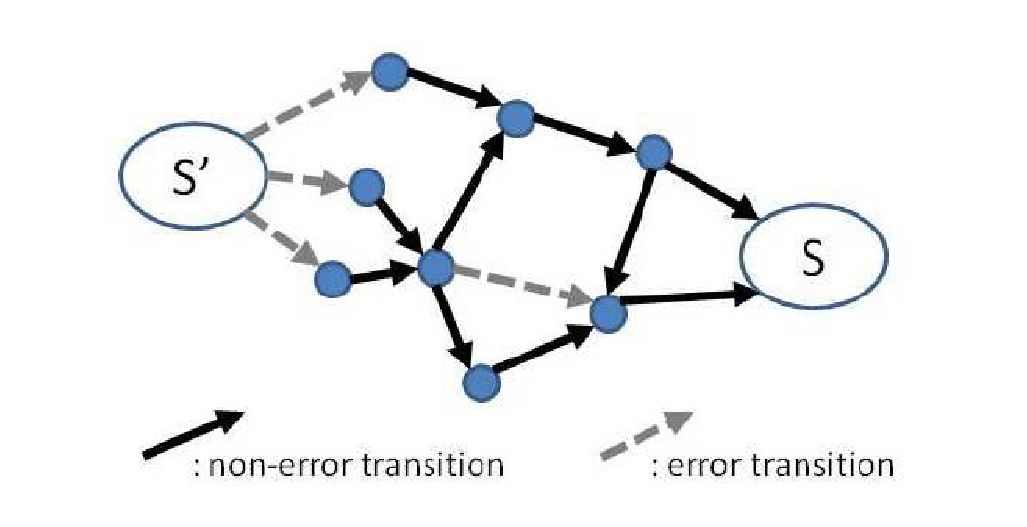
\epsfig{file=rseg.eps,width=60mm}
\caption{Illustration of the recovery operation}
\label{fig.sfrch} 
\end{center}
\end{figure}  
In this figure, the states in set $S'$ are computed  
as the precondition of states in $S$ through those transitions in the figure.  
Each path from $S'$ to $S$ is a recovery segment. 
$S$ and $S'$ may overlap.  
The blue circles represent states in the recovery segments.  
If we calculate $S'$ out of $S$, 
then, for each state $q'\in S'$, we can find a path from 
$q'\in S'$ via a path in the recovery segment to another state $q\in S$.  
The maximal number of errors in a recovery segment is 2.  
Thus the protagonist has a strategy to recover from errors in $S'$ to $S$ 
even when 2 errors happen in the corresponding recovery segment.  
When $S'=S$, then $S$ is a fixed point to the precondition 
operator through the recovery segments in the figure.  

Now we formally define the concept that we explained with Figure~\ref{fig.sfrch}.  

\begin{definition}{\bf ($k$-safety):} 
\label{k-safe}
Given a $k\in\nnneg$, 
a state $q$ is called \mbox{$k$-safe} with respect to 
a safety region $S\subseteq Q\smallsetminus F$ of non-failure states, 
denoted $q\in\safe_k(S)$, if there 
is a strategy for the protagonist to guarantee that 
we can reach back to $S$ from $q$, provided that
the overall count of errors is at most $k$.
\qed 
\end{definition}

However, the definition can be subtle in its interpretation.  
Specifically, the ability to stand against one wave of $k$ errors 
is not the same as that against repeated recovery 
from waves of $k$ errors.  
If the recovery mechanism is not designed properly, 
the system may gradually lose a bit of control after each wave of $k$ errors 
and eventually degrade to system-level failure. 

\begin{example} 
{\bf (Fault-tolerant computer architectures):}  
\label{exmp.avi.revisit}
Consider Example~\ref{exmp.avi} with $2k+1$ processor copies, 
with the objective to maintain majority checks
and to identify the bad processors. 
Indeed, according to the first, na\"ive solution, 
any safe state with a recovery strategy to 
$Q\smallsetminus F$ is good.   
After $k$ processor copies fail, 
the majority checks are still capable to maintain the correctness
of the combined behavior to follow the design of the original system.  
There seems to be nothing to do after $k$ errors.  
Thus, na\"ively, we can choose those states as the safety region
\label{reply1.majority.checks.as.safety.regions} if, 
at those states, majority checks still work.  

However, there is no expectation that the system will be able
to recover at any point in the future into a situation where it can bear 
another wave of $k$ errors.   
It will fail and lose the function of majority checks just after one more error.  
In contrast, in this work, we aim to propose a dense error resilience criterion that 
given no more errors for enough time to allow recovery, 
the system will eventually recover to resilience to $k$ dense errors again. 
%Note that `enough time' is a system parameter that refers to the time required for recovery, provided no further errors occur.
\qed 
\end{example} 

To look at this issue in more detail, 
please consider the transition system with four states, 
including a single failure state
(state $4$, marked by a double line) shown in Figure~\ref{fig:example}.
The controlled transitions are depicted as black solid arrows, 
the error transitions are depicted as red dashed arrows.
For $S=Q\smallsetminus F=\{1,2,3\}$, all states in $S$ are in $\safe_0(S)$.
For all $k \geq 1$, we have $\safe_k(S)=\{1,2\}$:
the protagonist can simply stay in $\{1,2\}$ 
during the safety phase of the game, and once the antagonist 
plays an error transition, the game progresses 
into the recovery segment, where the protagonist's objective 
is satisfied immediately.
This outlines the difference between $k$-sfrch-ty and 
the linear time property
of being able to repeatedly tolerate waves of up to $k$ errors, 
which would only be satisfied by states $1$ and $2$ for 
$k = 1$, and only for state $1$ for $k = 2$.



\begin{figure}[t]
\begin{center}
\psset{xunit=26mm,yunit=7mm}
\begin{pspicture}(0,-.15)(3,1.4)
% \pnode(0,.6){0}
\rput(0,0){\circlenode{1}{$1$}}
\rput(1,0){\circlenode{2}{$2$}}
\rput(2,0){\circlenode{3}{$3$}}
\rput(3,0){\circlenode[doubleline=true]{4}{$4$}}
% \ncline{->}{0}{1}
\nccircle{->}{1}{.35}
\nccircle{->}{2}{.35}
\nccircle{->}{3}{.35}
\ncarc[linecolor=red,linestyle=dashed]{->}{1}{2}
\ncarc{->}{2}{1}
\ncarc[linecolor=red,linestyle=dashed]{->}{2}{3}
\ncarc{->}{3}{2}
\ncline[linecolor=red,linestyle=dashed]{->}{3}{4}
\end{pspicture}
\end{center}
\caption{\label{fig:example} An example for calculating $\safe_k$}
\end{figure}




This difference raises the question 
if the rules of our game are depriving the antagonist 
of some of the $k$ errors that she should intuitively be allowed to insert in a wave.
The answer is that this is not the case 
if we use any fixed point of $\safe_k$ as $S$.
In this case, the protagonist would regain the capability to endure a wave of $k$ errors when reaching a safe state after recovery.
Instead of depriving the antagonist, 
one could say that we reset the number of errors in any recovery 
segment that the antagonist can inject to $k$.
Thus such a fixed point of $\safe_k$ should consist of 
states, from which we can use a control mechanism to fend off 
repetitive waves of $k$ dense errors in the recovery segments.  
For convenience, we call states in such a fixed point of $\safe_k$  
the $k$-resilient states. \label{reply1.k.resilient.states}  

% Thus, we can simply define the set of $k$-resilient states while the definition of $k$-sfrch-ty does not demand that the 
% system tries to recover, given enough 
% game steps, into a state where it can sustain more failures,
% for $k$-resilience, after recovery, $k$ more failures should be allowed, and so forth.
% Resilience is similar to the property of `home states', 
% where the system is capable, given enough time and 
% no interruption (in the form of failures), 
% of reaching again the good situation where it is again resilient to 
% $k$ failures.

For a state to be in $\safe_k(S)$, 
the system (protagonist) has a strategy to recover to $S$, 
given that a long enough execution commenced 
without another round of $k$ errors happening.
We say that two successive errors are in the same 
\emph{group of dense errors} 
if the sequence of states separating them 
was not long enough for recovery to the safety region.
Vice versa, if two successive errors are far enough apart 
such that the protagonist can guarantee recovery in this separation, 
then they do not belong to the same group.
% (Besides the practical motivation of what recovery encounters in our examples, this assumption also has the technical motivation that memoryless strategies suffice for the protagonist to win $\safe_k(G)$.)
% 
% A state is $k$-resilient if groups of up to $k$ dense failures can be tolerated infinitely many times, provided that the system is given enough time to recover;
% $k$-sfrch-ty is equivalent to tolerating up to {\em one} set of $\leq k$ dense errors%
% \footnote{Note that the technical definition of sfrch states implies that a set of dense errors ends once the protagonist has recovered to $G$.
% Thus, as seen in the example, a state from which no two failures can be tolerated might be $k$-sfrch for all $k$.}.

To check whether recovering to $S$ by the protagonist (the fault-tolerance mechanism)
is always possible, provided that at most $k$ errors occurred during 
a recovery segment, observe that nesting 
$\safe_k$ once, i.e., $\safe_k(\safe_k(\cdot))$, corresponds
to tolerating up to two rounds of up to $k$ dense errors, and so forth.
Thus, for $S$ to be a target of recovery for $k$-resilience, 
$S$ must be a fixed point of the operator
$\safe_k$ from Definition~\ref{k-safe}, or, equivalently, 
$S=\safe_k(S)$ must hold.  
Moreover, if $S$ is the greatest fixed point to $k$-resilience, then we we can apply 
$\safe_k()$ any number of times to $S$ and still obtain $S$.  
Computationally, the greatest fixed point of $\safe_k$ can be constructed as 
by executing  
\begin{center} 
$\safe_k(\safe_k(\safe_k(\ldots\ \safe_k(S\big)\ldots)))$,
\end{center}  
using a sufficiently deep nesting that a fixed point is reached.

Note that this fixed point $x$ to $x=\safe_k(x)$ is what we are really interested in, 
while $\safe_k(S)$ for a given $S$ is an intermediate result that does not 
guarantee survival of the systems after waves of dense errors.
If this greatest fixed point
$$R = \bigcup\{X \subseteq S \mid X = \safe_k ( X )\}$$ is non-empty, 
the protagonist's strategy for 
the fixed point (guaranteeing eventual recovery 
to a state in the fixed point within no more than $k$ errors, i.e., $k$-resilience) 
can be used to control the recovery mechanism, 
constraining its transitions to follow its winning strategy.

As explained in the introduction, 
there can be several natural control problems in our safety resilience game.
First, the system designers may want to know whether the chosen safety region $S$ can 
be supported by the recovery mechanism for resilience level $k$.  
Second, they may want to get design support for choosing the safety region 
for achieving resilience level $k$.  
Finally, they may want to know the maximal resilience level that they can achieve. 


With the explanation in the above, in the rest of the manuscript, 
we will focus on the algorithm for constructing 
$\safe_k(\cdot)$ and evaluating $k$-resilient states. 




\section{Safety resilience games \label{sec.rgame}} 

A system is $k$-resilient if it
can be controlled to tolerate infinitely many groups of up to $k$ dense errors, 
provided that the system is given enough time to recover between these groups.
As we have explained, in systems developed with defensive mechanism against errors,  
when errors are detected, recovery procedures should be activated.  
The major challenge is to decide given a set of failure states and a safety region,
whether 
the recovery mechanism can support a resilience level required\label{reply1.prescribed.2.required} by the users. 
Our goal is to develop techniques with a solid foundation to 
assist the system designers in evaluating the resilience of their systems, 
to synthesize the controller strategy for the required resilience level, and 
to achieve the maximal resilience level. 


We now formally define the safety resilience game played between a 
system (the protagonist) and an error-injector (the antagonist).  
Initially, the two players are given a 2-player concurrent game structure $\calk$,  
a pebble in $r$,  
a set $F\subseteq Q$ of failure states, and 
a safety region $S\subseteq Q\smallsetminus F$. 
Then the recovery region consists of states in $Q\smallsetminus (F\cup S)$.  
The two players together make decisions and move the pebble from state to state.   
The antagonist tries to deflect a play into $F$ by injecting sufficiently many errors, while
% On the other hand, 
the protagonist tries to avoid that the pebble reaches $F$. 
To achieve this, the protagonist can use the recovery region as the safety buffer and try to 
get back to $S$ as soon as the play is deflected from $S$ 
to the recovery region.  
If a system is resilient to $k$ errors, then it means that 
the protagonist can handle up to $k-1$ errors while in the recovery region.  
Thus when checking whether a system is resilient to $k$ errors, 
we only need to check those recovery segments with no more than $k-1$ errors. 

In the following, we formalize the concept.  

\begin{definition} \label{def.srgs} 
{\bf (Safety resilience game structure):} 
Such a structure is a pair $\langle \calk, F\rangle$ with the following 
restrictions. 
\begin{list1} 
\item $\calk$ is a 2-player concurrent game structure 
  $\langle Q,r,P,\lambda,E_1,E_2,\delta\rangle$.  
  Conceptually, the first player represents the system / the protagonist, while 
  the second player represents the error model / the antagonist.  
\item $E_2$ is partitioned into error and and non-error moves $E_{\emerr}$ and $E_{\emnerr}$, respectively.
%   The error moves are characterized by a condition `$\emerr$', while the non-error moves  are characterized by a condition `$\emnerr$'.
We require that only the 2nd player can issue $\emerr$ moves.  
Moreover, $E_{\emnerr}$ must be non-empty. 
\item $F$ is the set of failure states in $Q$ with $r\not\in F$.   
\end{list1} 


The antagonist can choose if she wants to respond on a move of the protagonist with an error move. \label{abstraction}
We allow for different non-error moves to reflect `normal' nondeterministic behavior, e.g., caused by abstraction. 
We allow for different error moves to reflect different errors that can occur in the same step.

We sometimes refer\label{reply1.reffer} to transitions with $\emerr$ moves by the antagonist as \emph{error transitions} and 
to transitions with  $\emnerr$ moves by the antagonist as \emph{controlled transitions}.  

For a party $A \subseteq \{1,2\}$, we refer with $\overline{A} = \{1,2\} \setminus A$ to the players not in the party, and by $E_A$ to the moves made by the players in $A$, that is, $E_{\{1,2\}} = E_1 \times E_2$, $E_{\{1\}} = E_1$, etc.

% For convenience of algorithm explanation, we require that $\delta$ is 
% a total function.  
% This does not compromise the expressiveness of $\calk$ for 
% modeling undefined moves since we can create an auxiliary failure state in $F$ 
% revise $\calk$ so that all undefined moves end at this failure state. 

The antagonist can use both error and non-error moves to influence the game.
In a simple setting, the antagonist may only have the choice to insert error-moves, while there is only a single controlled transition.
In this simple case, the protagonist can choose the successor state alone unless the antagonist plays an error transition.  
% Such simple systems can be useful in simplifying the error models. 
Specifically, a safety resilience game structure is {\em simple} if $E_2$ contains only one error move.
\label{reply1.2.complexities} 
Considering simple safety resilience game structures leads to lower 
complexities, as it changes reductions from reachability in games (PTIME-complete \cite{Immerman81})
to reachability in graphs (NL-complete \cite{Papadimitriou94}).
% % the 
% % following two conditions are satisfied. 
% % \begin{list1} 
% % \item There are only two moves that the antagonist can issue, 
% %   the $\emerr$ move (representing a system error) and 
% %   the $\emnerr$ move (representing no system error). 
% % \item The destination states of error transitions are independent of   
% %   the moves selected by the protagonist.  
% %   \qed 
% % \end{list1} 
% 
% \pagebreak \pagebreak
% Thus, we require that, for every state $q$ and 
% every move vector $[e_1,e_2]$, the following constraints are true. 
% \begin{list1} 
% \item If $e_1\in\{\emerr,\emnerr\}$, then $\delta(q,e_1,e_2)=\perp$. 
% \item If $e_2\not\in\{\emerr,\emnerr\}$, then 
%     $\delta(q,e_1,e_2)=\perp$. 
% \item For every state $q\in Q\smallsetminus F$, there exists an $e\in E$ with 
%   $\delta(q,e,\emnerr)\neq \perp$.  
%   This means every functional state has a controlled successor when no 
%   error occurs.  
\qed 
% \end{list1} 
\end{definition} 

Note that, in the game structure, only one system player and one error model player 
are allowed.   
This is purely for the simplicity of algorithm presentation.  
With proper reduction techniques, we can easily convert 
a game structure with more than one system player and 
more than one error model player to the structure in Definition~\ref{def.srgs}.  
The standard technique would be using the transition rules of 
the product automata of the system players for the protagonist while 
using the transition rules of the product automata of the error model players 
for the antagonist.  
In fact, we indeed use this reduction technique in our experiment for 
analyzing the resilience levels of multi-agent systems.  

From now on, we assume that we are in the context of a 
given safety resilience game structure $\calg=\langle \calk,F\rangle$. 

\begin{definition}\label{def.rec.seg}
{\bf (Recovery segements):} 
We need to rigorously define {\em recovery segments}. 
A play prefix $\rho$ is a {\em recovery segment} to safety region $S\subseteq Q\smallsetminus F$ 
if it satisfies the following constraints. 
\begin{list1} 
\item %$\rho(0)=r$ or
      $\rho(0)\in S$. 
\item If $|\rho|=\infty$, then all states in $\rho[1,\infty)$ are 
  in $Q\smallsetminus(S\cup F)$. 
  In this case, $\rho$ is called a failed recovery segment. 
\item If $|\rho|\neq \infty$, then all states in $\rho[1,|\rho|-2]$ 
  are in $Q\smallsetminus(S\cup F)$ and 
  $\emlast(\rho)=\rho(|\rho|-1)$ is either in $F$ or $S$.    
  If $\emlast(\rho)\in F$, $\rho$ is also a failed recovery segment; 
  otherwise, it is a successful one. 
\end{list1} 
We use $\mbox{\em level}(\rho, S)$ to 
denote the number of error moves between states in $\rho$  
with respect to the safety region $S$:
$\mbox{\em level}(\rho, S) \defn \big\lvert\{i \in [0,|\rho|-1) \mid \rho_e(i) \models E_{\emerr}\}\big\rvert$.
\qed 
\end{definition} 

As stated in the introduction, we propose 
a game-theoretic foundation for resilience analysis of software systems. 
With this perspective, the protagonist acts as a maximizer, who wants to maximize the 
resilience levels along all plays.
For this, the protagonist fixes a strategy that describe what he is going to do on each play prefix.
The antagonist acts as a minimizer, who wants to minimize the resilience level.
She can resolve nondeterminism and inject errors in order to achieve this, and (although this plays no major role in this setting) she knows the strategy the protagonist has fixed and can use this knowledge in principle.

The goal of the protagonist is therefore the same as the goal of the system designer: to obtain a strategy that offers a maximal level of resilience in a safety game. 
\label{reply1.memoryless.unbounded.resilience} 
However, in order to avoid degenerate behavior where the protagonist benefits from being in the recovery phase and from the antagonist therefore being allowed less errors in the current wave of errors she may inject, we have to strengthen his obligation to eventually recover to the safe states when the environment chooses not to inject further errors.
This way, the protagonist has no incentive to cycle in the recovery region.
Consequently, he can recover to the safe region within $|Q|$ moves after the antagonist has inserted the last error of the current wave, irrespective of whether the antagonist would be allowed to insert further errors in this wave.
This is the key reason why memoryless optimal control exists for this error model, why it is reasonable to assume swift recovery, and, consequently, why it is a posteriori justified to leave the separation time between two waves implicit: the time to traverse $|Q|$ states suffices.

% this we have to be careful to define the goal rigorously 
% so that the protagonist may not choose to stay in a successful recovery segment, 
% watch the antagonist committing unboundedly many error moves, 
% and only then choose to leave the recovery segment. 
% Such degenerate scenarios are avoided in our theoretical foundation 
% since our transition function is a total function from events to 
% the destination states.  
% Thus as long as $E_2$ does not contain only the error move, then 
% there is always an non-error transition from every state.  

% Likewise, if the antagonist can deflect a play to failure, then she must be
% able to do this in $|Q|$ moves.  
% Since the antagonist is a minimizer of the resilience level in 
% the game, then, if the antagonist cannot direct a play to failure with 
% $|Q|$ errors in the recovery segment, it simply will 
% not inject any error to admit the resilience level to grow 
% unboundedly.  

Besides obtaining this from intuition, we can also consider the tree of successful recoveries for any protagonist strategy that can endure $k$ error moves by the antagonist.
The tree of recoveries from up to $k$ errors is finite according to 
the definition of successful recovery segments. 
Then for any subtree $t$ in this tree of recoveries with a node $v$ in $t$ 
such that $v$ is labeled with the same state as the root of $t$ with no error on the path,   
we can always replace $t$ with the subtree rooted at $v$.  
After the replacement, we have a tree of recoveries with no greater depth than 
the original one. 
After repeating such replacements, 
this immediately provides a translation from such a strategy with unrestricted memory 
to one with memory of size $k$ (the resilience level).
The restriction to memoryless strategies follows from the construction we give 
in Section~\ref{sec.mck}, 
which does not depend on the memory and still yields a strategy, which is memoryless.
Thus, in this work, we should define the resilience level of software systems based 
on \emph{memoryless} protagonist strategies.  

Based on the argument above, 
the gain of the protagonist in a play can be defined as follows. 

\begin{definition}
\label{def.gain} {\bf (Gain):} 
Given safety region $S \subseteq Q\smallsetminus F$, 
the gain of a play $\rho$ to $S$, in symbols $\emgain(\rho,S)$, 
denotes the maximal integer $k \in \mathbb N$ such that, 
for all recovery segments $\rho_r$ to $S$ in $\rho$, 
if $\mbox{\em level}(\rho_r,S)\leq k$, 
then $\rho_r$ is a successful recovery segment to $S$. 
\qed 
\end{definition}

The resilience level of a safety resilience game is defined 
as the maximum gain that the protagonist can guarantee in all plays 
with a memoryless strategy.  


%  
% Given a safety region $S$ and a play $\phi$ in $\calk$, 
% the gain of the protagonist in $\phi$ with respect to $S$, 
% in symbols $\emgain(\phi,S)$, 
% is defined as the maximum $k\in\nnneg$ such that 
% every recovery segment in $\psi$ with respect to $S$ 
% with no more than $k$ errors are successful. 

\begin{definition}\label{def.srgame}  
{\bf (Safety resilience game):} 
Such a game is zero-sum and defined on 
a safety resilience game structure $\calg=\langle \calk,F\rangle$ 
and a safety region $S\subseteq Q\smallsetminus F$. 
The gain of $\calg$ to $S$, in symbols $\emgain(\calg,S)$, is defined as 
the maximum gain that the protagonist can manage with memoryless strategies.  
Rigorously, 
\begin{center} 
$\emgain(\calg,S)\defn \max_{\sigma\in \Sigma^{(0)}}\min_{\sigma'\in \Sigma}
\emgain(\emplay(r,\sigma,\sigma'),S)$
\end{center} 
\label{reply1.emplay} 
Please be recall that $\emplay(r,\sigma,\sigma')$ is the play from $r$ 
according to strategies $\sigma$ and $\sigma'$ respectively of the 
two players. 
Moreover $\Sigma^{(0)}$ is the set of memoryless strategies. 

We say that the resilience level of $\calg$ to $S$ is $\emgain(\calg,S)$. 
\label{reply2.optimal}
A strategy $\omega$ for the protagonist is optimal to $S$ if 
$\min_{\sigma'\in \Sigma}
\emgain(\emplay(r,\omega,\sigma'),S)=\max_{\sigma\in \Sigma^{(0)}}\min_{\sigma'\in \Sigma}
\emgain(\emplay(r,\sigma,\sigma'),S)$.  
When $S$ is not given, 
we say that $\calg$ is {\em $k$-resilient} if there exists a non-empty $S \subseteq Q \setminus F$ with $\emgain(\calg,S)\geq k$.
\qed 
\end{definition} 

\paragraph{\bf Remark.}\hspace*{-2ex}
While the option of using memoryless strategies plays a minor role in the technical argument, it plays a paramount role in the usefulness of the resulting control strategy:
choosing memoryless strategies implies that all recovery segments are short.
In particular, all sub-paths (recovery segments) between two waves of dense errors injected by the antagonist are shorter---and usually significantly shorter---than the size of $\calg$.
In consequence, any time span long enough for traversing the recovery segment will lead to a full recovery.
It is therefore sufficient for a temporal distance we have to assume between two waves of dense errors.







\section{Alternating-time $\mu$-calculus with events (AMCE)  
\label{sec.amc}
} 


We propose to solve our resilience game problems with an 
existing technology, i.e., model-checking of alternating-time $\mu$-calculus 
({\em AMC}) formulas.  
AMC is a propositional temporal logic 
with fixed point operators.  
For example, the following formula 
\begin{center} 
\hfill 
$\mu X.(\text{\em safe}\vee \langle 1\rangle \nxt X)$
\hfill (A) 
\end{center} 
uses least fixed point operator $\mu$ to declare a fixed point variable 
$X$ for a set of states. 
Subformula $\langle 1\rangle \nxt \phi$ existentially 
quantifies over 
the protagonist strategies that can direct the plays to a successor state 
satisfying $\phi$.  
Together, the formula specifies a set $X$ of states that can inductively reach a safe 
state with the control of the protagonist. 
Specifically, the formula says that a state is in $X$ if 
either it is {\em safe} 
or the protagonist can direct to a successor state known to be 
in $X$.  
For our game structures, we only need strategy quantification 
of up to two players.  

However, we need extend AMC with some simple syntax sugar.  
There are two extensions.  
The first is for Boolean combinations of path modalities in the 
scope of strategy quantification. 
For example, the following AMCE formula 
\begin{center} 
\hfill 
$\langle 1\rangle((\mbox{\em smoke}\Rightarrow\nxt\mbox{\em alarmOn})\vee 
\nxt\mbox{\em windowClosed})$ 
\hfill (B) 
\end{center} 
says that the protagonist can enforce either of 
the following two path properties with the same strategy. 
\begin{list1} 
\item If there is smoke, then the alarm will be turned on in the next state. 
\item The window will always be closed in the next state.  
\end{list1} 
Such a formula is not in ATL and AMC \cite{AHK02}.  

The second extension is for restricting transitions that may participate 
in the evaluation of path formulas.  
The restriction is via constraints on moves on transitions and 
can, in our extension to AMC, be specified with a  
move symbol set to the next-state modal operators.  
For example, the following AMCE formula  
\begin{center} 
\hfill $\langle 1\rangle ((\nxt^{2:\emserr}\mbox{\em alarmOn}) 
\wedge (\nxt^{\neg 2:\emserr}\neg\mbox{\em alarmOn}))$ 
\hfill (C) 
\end{center} 
says that the protagonist can 
\begin{list1}
\item turn on the alarm when an error occurs; and 
\item keep the alarm silent when no error occurs.
\end{list1} 
Before we formally present AMCE, we need define expressions for 
constraints on moves of players in transitions.  
We adapt an idea from \cite{Wang14}.  
Specifically, a {\em move expression} $\eta$ is of the following syntax. 
\begin{center} 
$\eta ::= a:e \mid \eta_1\vee\eta_2 \mid \neg \eta_1$
\end{center} 
Here, $a$ is a player index in $\{1,2\}$ and $e$ is a move symbol in $E_1\cup E_2$.  
$\vee$ and $\neg$ are standard disjunction and negation.  
% $\true$ can be seen as a shorthand of $1:E$.  
Typical shorthands of Boolean operations can also be defined out of 
$\vee$ and $\neg$.  
A total move vector can be expressed as $[e_1,e_2]$ 
where for all $a\in\{1,2\}$, $e_a\in E_a$ is the move by 
player $a$ specified in the vector.  
We say $[e_1,e_2]$ satisfies $\eta$, in symbols 
$[e_1,e_2]\models \eta$, if and only if the 
following constraints are satisfied. 
\begin{list1} 
\item $[e_1,e_2]\models a:e$ if, and only if, $e_a$ is $e$.  
\item $[e_1,e_2]\models \eta_1\vee\eta_2$ 
  if, and only if, $[e_1,e_2]\models \eta_1$ or 
  $[e_1,e_2]\models \eta_2$. 
\item $[e_1,e_2]\models \neg\eta_1$ 
  if, and only if, $[e_1,e_2]\not\models \eta_1$.   
\end{list1} 



\subsection{Syntax\label{subsec.syntax}}



 
A formula $\phi$ in AMCE has the following syntax. 
\begin{center} 
$\begin{array}{rrl} 
\phi	& ::= & p 
	\mid X 
	\mid \phi_1 \vee \phi_2
	\mid \neg \phi_1 
 	\mid \mu X.\phi_1 
 	\mid \langle A\rangle \psi\\ 
\psi	& ::= &
	\mid \psi_1 \vee \psi_2
	\mid \neg \psi_1 
 	\mid \nxt^\eta \phi_1
\end{array}$ 
\end{center} 
Here, $\phi$ is a state formula, $\psi$ is a path formula,  
$p$ is an atomic proposition symbol in $P$ 
(atomic proposition set, as in Definition~\ref{def.cncgame})\label{reply1.P.x}, 
and 
$X$ is a set variable for subsets of $Q$.
The Boolean connectors are the common ones: $\vee$ for disjunction and 
$\neg$ for negation.
Note that we allow for Boolean combinations of the next operators $\nxt$ 
under strategy quantification  $\langle A\rangle$.  
This is one major difference of AMCE from AMC.  

Formula $\mu X.\phi_1$ is the usual least fixed point operation to $\phi_1$.
According to the tradition in \cite{AHK02}, 
we require that all free occurrences of $X$ in $\phi_1$ must occur
within an even number of scopes of negations.    
This is because sentences with a negative occurrence, like $\mu X. \neg X$, have no natural semantics.
A set variable $X$ is {\em bound} in a formula $\phi$ if it is inside a declaration scope of $X$.  
If it is not bound, then it is {\em free}.  
An AMCE sentence is an AMCE state formula without free set variables. 
In most cases, we are interested in specifications given as AMCE sentences.  


The $A$ in $\langle A \rangle$ is a finite set of player indices 
in $[1,2]$.
Conceptually, $\langle A \rangle\psi$ means that players in $A$ can collaborate 
to make $\psi$ true. 
For example, $\langle \{1,2\}\rangle\nxt p$ means that 
players~1 and~2 can collaborate to make $p$ true in the next state. 
We follow the notations in \cite{AHK02} and omit the parentheses in 
formulas like $\langle A\rangle \psi$.  
For example, $\langle \{2\}\rangle \nxt p$ 
and $\langle \{1,2\}\rangle \nxt p$ 
will be abbreviated as 
$\langle 2\rangle \nxt p$ and   
$\langle 1,2\rangle \nxt p$ respectively.  

We allow event 
restrictions as superscripts in $\nxt^\eta\phi_1$ 
with a move expression $\eta$.  
The operator is important in supporting the evaluation of safety resilience levels with traditional model-checking technology.  
Note that since AMC \cite{AHK02} only allows for the next-state temporal 
modality, 
only the choice of moves to the next states of a strategy matters.  
Formula $\nxt^\eta\phi_1$ is thus evaluated at states  
with respect to move vectors satisfying constraint $\eta$.  
The formula is true of a move vector $[e_1,e_2]$ if and only if 
$[e_1,e_2]\models \eta$  
implies the satisfaction of $\phi$ at state $\delta(q,e_1,e_2)$. 
Also 
$\nxt^{1:E_1}\phi_1$ can be written as $\nxt\phi_1$ in AMC \cite{AHK02} 
and 
the superscript to $\nxt$ can be omitted.    



We also adopt shorthands in the below.  
The $\beta$ refers to state or path formulas.
\begin{center} 
$\begin{array}{rcl}
\true	& \defn & p \vee \neg p \\
\false	& \defn	& \neg p \wedge p \\ 

\beta_1 \wedge \beta_2 & \defn & \neg((\neg \beta_1) \vee (\neg \beta_2)) \\ 
\beta_1 \Rightarrow \beta_2 & \defn & (\neg \beta_1) \vee \beta_2 \\

\nu X.\phi & \defn & \neg \mu X.\neg\phi \\ 

{[A]\psi} & \defn & \neg \langle A\rangle \neg\psi \\ 
\end{array}$
\end{center} 





\subsection{Semantics \label{sec.amc.semantics}} 

In the following, we adapt the presentation style of \cite{AHK02} 
to define the semantics of AMCE inductively over the structure of the subformulas.  
The value of a state formula at a state \label{reply1.semantics.dont.understand} 
is determined by the interpretation of the set variables.  
Such an interpretation $I$ maps set variables to subsets of $Q$.  
In comparison, the value of a path formula at a state 
is determined by both the interpretation
of the set variables and the move vector chosen by the players. 
For convenience and conciseness of presentation, 
we extend the definition of interpretation of \cite{AHK02} also to 
record the chosen move vector by some players. 
Specifically, we use an auxiliary variable ``$\move$"  
for the present chosen move vector in the evaluation of path formulas. 
Given an interpretation $I$, $I(\move)$ records the chosen move vector  
of all players in $I$.  
For example, $I(\move)=[\text{\tt setAlarm},\perp]$ 
means the chosen move vector 
that player 1 sets on an alarm while player 2 does nothing under interpretation $I$. 

We need the following concept for collaborative choices of moves 
to the next states by some players. 
An {\em enforced move vector set} by $A\subseteq [1,2]$ is 
a maximal set of move vectors that agree on the choices of moves 
by players with indices in $A$. 
Specifically, given an enforced move vector set $C$ by $A$, 
we require that, for every $[e_1,e_2]\in C$,  
$[e'_1,e'_2]\in C$, and $a\in A$, $e_a=e'_a$.  
For convenience, we let $\Gamma^A$ denote the set of all 
enforced move sets by $A$.  

Following the semantics style of \cite{AHK02}, 
we can extend $I$ to be an interpretation of all state and path formulas.  
Intuitively, given a state or path formula $\beta$, 
$I(\beta)$ is the set of states that satisfy $\beta$ according to
the assumption on values of set variable values and auxiliary 
variable ``$\move$."
More precisely, 
$I(\beta)$ is a subset of $Q$ 
that satisfies the following inductive rules. 
\begin{list1} 
\item $I(p)=\{q\mid p\in \lambda(q)\}$. 
\item $I(\beta_1\vee\beta_2)=I(\beta_1)\cup I(\beta_2)$. 
\item $I(\neg\beta_1)=Q-I(\beta_1)$.

\item $I(\mu X.\phi_1)$ is the smallest set $Y\subseteq Q$ 
  with $Y=I[X\mapsto Y](\phi_1)$, where 
  $I[X\mapsto Y]$ is a new interpretation identical to $I$ 
  except that $X$ is interpreted as $Y$.

\item $I(\langle A\rangle \psi)$ is the set of states 
such that there is an enforced move vector set $C$ by $A$ such that, for all move vectors $\epsilon \in C$,  
  $I[\move\mapsto \epsilon](\psi)$ holds:
  \begin{center} 
  $I(\langle A\rangle \psi) = 
  \bigcup_{C \in\Gamma^A}
  \bigcap_{\epsilon \in C} I[\move\mapsto \epsilon](\psi)$ 
  \end{center} 
\item Given $I(\move)=[e_1,e_2]$, 
  if $[e_1,e_2]\models \eta$, then  
$I(\nxt^\eta \phi_1) = \{q \in Q \mid \delta(q,e_1,e_2) \in I(\phi_1)\}$; 
otherwise $I(\nxt^\eta \phi_1) = Q$.  

\end{list1} 
A concurrent game structure is a model of an AMCE sentence $\phi$, if its initial state $r$ is in the interpretation of $\phi$ ($r \in I(\phi)$) for any interpretation $I$.

Note that, strictly speaking, AMCE does not add much to the 
expressiveness of AMC.  
In the literature, propositions have often been used to 
record events.  
Intuitively, we would need one atomic proposition for each event to mark that it has just occurred.
This event marker would be true exactly at states right after the event happened. 
(One would possibly have to create multiple copies of states to reflect this.)
 
As discussed in \cite{Wang04}, such a modeling technique leads to an unnecessary 
blow up of the state space, which could be exponential in the number 
of players in general concurrent games.  
\label{reply1.event.blowup} 
By properly selecting 
the transitions with respect to operators like $\nxt^\eta$, 
such auxiliary propositions are not necessary when encoding the state space.  
Thus, AMCE can also be of interest to practitioners for the
efficient analysis and verification of general concurrent games.





\section{Resilience level checking algorithm \label{sec.mck}}
\label{sec:kresil}

In Subsection~\ref{subsec.ideas}, we have proposed the 
idea of the $\safe_k(\cdot)$ operator and proposed 
to use its greatest\label{reply2.empty.fixed point} fixed point 
for the evaluation of $k$-resilience.
In the following, we first establish some properties of $k$-safety 
and then use AMC model-checking technology to solve the 
safety resilience games.  


\subsection{High-level description of the algorithm} 

The following lemma shows the sufficiency of $k$-safety as a building block for 
solving safety resilience games.

\begin{lemma} 
\label{fixed point}
For a safety resilience game $\calg$, 
$\safe_k(\cdot)$ has a greatest fixed point.
\end{lemma}
\pf 
The lemma follows from the facts that
the function $\safe_k$ is monotonic
($S \subseteq S'$ implies $\safe_k ( S ) \subseteq \safe_k ( S' )$ 
because a winning strategy for the protagonist 
for $S$ is also a winning strategy for $S'$ 
for all states in $\safe_k(S)$) and operates on a finite domain.
\qed


For the example in Figure~\ref{fig:example}, 
considering $S=\{1\}$ ($\{1\}=\safe_2(\{1,2,3\})$), 
the only state in $S$, state $1$, is $2$-resilient: 
it can recover with the recovery strategy to always go to the left.

The set of $k$-resilient states of $\calg$, 
can be calculated as the greatest solution to 
$S=\safe_k(S)$ with $S\subseteq Q\smallsetminus F$. 
Technically\label{reply2.technically.comma} we can start the inductive calculation of the greatest fixed point 
from base case $S_0 = Q \smallsetminus F$, 
and successively calculate $S_{i+1} = \safe_k(S_i)$, 
for each $i\geq 0$. 
The set of $k$-resilient states is then the limit $S_\infty$.  
As soon as we have $S_{i+1}=S_i$, a fixed point is reached.
We then have $S_i=S_\infty$ and can stop the 
inductive construction.  
Since $S_0$ is finite and $S_{i+1}\subseteq S_i$ holds for all $i\geq 0$, 
we will eventually reach a $j$ with $S_{j+1}=S_j=S_\infty$. 









\subsection{Realization with AMCE model-checking 
\label{subsec:kSafety}
}

We need formally define the interaction among strategies of players. 
We borrow the notation of function composition. 
Given two partial functions $\beta_1$ and $\beta_2$, 
we use $\beta_1\circ \beta_2$ to represent their composition.  
Specifically, we have the following definition.  
\begin{center} 
$\beta_1\circ\beta_2(a)=\left\{\begin{array}{ll} 
\beta_1(a) & \mbox{ if } \beta_2(a)\mbox{ is undefined}.\\
\beta_2(a) & % \mbox{ if } \beta_1(a)\mbox{ is undefined}.  \\
% \mbox{undefined} & 
\mbox{otherwise} 
\end{array}\right.$
\label{reply1.compose} 
\end{center} 
% Note that, if $a$ is defined in both $\beta_1$ and $\beta_2$, 
% then $\beta_1\circ\beta_2(a)$ is undefined. 
% 
For our purpose, a partial strategy vector is a mapping from $\{1,2\}$ to $\Sigma$ 
and can be undefined for some players in $\{1,2\}$.  
It is for a party $A\subseteq \{1,2\}$ if it is defined only for players in $A$
and represents a collaborative strategy of the players with a 
defined strategy in $A$.  
It is total if it is defined for all players.  


For convenience, we also define partial move vectors 
as mappings\label{reply2.mapping.s} from $\{1,2\}$ to $E$.  
A partial move vector is for a party $A\subseteq\{1,2\}$ if it is defined only for players in $A$.  
It is total if it is defined for all players in $\{1,2\}$.  
Given two partial move vectors $\gamma_1$ and $\gamma_2$, \label{reply1.m2gamma} 
we define $\gamma_1\circ\gamma_2$ to represent the composition of 
the two vectors.  

Given an $S$, 
we propose to construct $\safe_k(S)$ in an induction on\label{induction.on.k} $k$.  
We need the following preliminary concepts for the presentation. 


\begin{definition} 
\textbf{(Traps)}
\label{def.traps}
For $A\subseteq \{1,2\}$,
a {\em trap} for $A$ is a subset $Q'\subseteq Q$ 
that party $\{1,2\}\smallsetminus A$ has a strategy vector $\beta$ 
to keep all plays from leaving $Q'$.  
Formally, we require that, for every $q\in Q'$ 
and partial move vector $\gamma$ for $A$, 
there exists a partial move vector $\gamma'$ for $\{1,2\}\smallsetminus A$ 
such that $\delta(q,\gamma\circ\gamma'(1),\ldots,\gamma\circ\gamma'(m))\in Q'$. 
\qed
\end{definition}




\subsubsection{Base case, $\safe_0(S)$} 

In the base case, 
$\safe_0(S)$ characterizes those states, from which the protagonist 
can direct the plays to 
$S$\label{reply2.those.states.that.can.goto.S}   
 and 
stay there via a protagonist strategy when there is no error injected by 
the antagonist. 
Thus $\safe_0(S)$ is the greatest trap for the antagonist to $S$ when no error happens and 
the greatest solution to the following equation. 
\begin{center} 
\label{reply2.SPrime}
$X=\left\{q \left| \begin{array}{l}
	q\in X\cap S, e\in E_1, \\
	\forall e'\in E_2(e' \neq \emnerr\Rightarrow \delta(q,e,e') \in X) 
	\end{array}\right.\right\}$. 
\end{center} 
In AMCE, we can alternatively define $\safe_0(S)$ as follows. 
\begin{center} 
\label{reply2.smallX}
$\safe_0(S)\defn \nu X.(S\wedge\langle 1\rangle \nxt^{\neg 2:\emserr} X)$.  
\end{center} 
This is the usual safety kernel of $S$, which consists of those states, from 
which any controlled transition is safe.  
It can be computed by the usual greatest fixed point construction.

\begin{lemma}
\label{lem:NLSafe0}
$\safe_0(S)$ can be constructed, together with a suitable memoriless
control strategy, in time linear to the size of $\calg$.
\end{lemma}
\pf 
A state $q\in S$ can stay in $\safe_0(S)$ if there is a choice $e\in E_1$ 
such that for all $f\in E_2$, $\delta(q,e,f)\in \safe_0(S)$.  
Basically, we can use the typical approach of iterative elimination 
to calculate $\safe_0(S)$. 
That is, we first let $K_0=Q-S$.  
Then we a sequence of mutually disjoint sets 
$K_1,K_2,\ldots,K_i,\ldots$ such that 
for all $i\geq 1$, states in $K_{i+1}$ can be shown to be not 
in $\safe_0(S)$ by evidences of states in $K_i\cup \ldots\cup K_0$.    
Linear time can be achieved with careful book-keeping of the choices of 
moves at all states in $S$. 
We need a counter $c_q$ for each $q\in S$ initialized to 
$|E_1|$ for the initial number of candidate choices of moves. 
Then for each $[q,e]\in S\times E_1$, we need a Boolean flag $b_{[q,e]}$ 
initialized to $\true$ to represent that 
$\{[e,f]\mid f\in E_2\}$ is still a valid choice of moves at $q$ to 
satisfy $\safe_0(S)$. 
For each state $q$, we also need to maintain a list of transition source states. 
That is, for each $\delta(q',e,f)=q$, we need 
record $[q',e,f]$ in list $L_q$.  
Then the iterative elimination proceeds as the algorithm in 
table~\ref{tab.safe0}.  
\begin{table}[!t]
\caption{Algorithm for $\safe_0(S)$ by iterative elimination} 
\label{tab.safe0}
\procbegin \noindent 
$\safe_0(S)$  
\begin{algorithmic}[1]
\FORNLINE {$q\in S$} $c_q=|E_1|$ \ENDFORLINE 
\FORNLINE {$q\in S, e\in E_1$} $b_{[q,e]}=\true$ \ENDFORLINE 
\STATE Let $i=0$ and $K_0=Q-S$. 
\WHILE {$K_i\neq \emptyset$} 
  \STATE Let $K_{i+1}=\emptyset$. 
  \FOR {$q\in K_i$ and $[q',e,f]\in L_q$} 
    \IF {$b_{[q',e]}$ is $\true$} 
      \STATE Let $c_{q'}=c_{q'}-1$. 
      \IFNLINE {$c_{q'}$ is $0$} add $q'$ to $K_{i+1}$.  \ENDIFLINE  
    \ENDIF 
    \STATE Set $b_{[q',e]}$ to $\false$. 
  \ENDFOR
  \STATE Increment $i$ by $1$.  
\ENDWHILE 
\RETURN $S-(K_0\cup \ldots \cup K_i)$.  
\end{algorithmic}
\procend 
\end{table} 
The algorithm is linear time since each transition $\delta(q,e,f)$ is 
checked exactly once. 
\qed

\subsubsection{Inductive cases, $\safe_k(S)$} 

Now we explain how to define the inductive cases of $\safe_k(S)$. 
The condition is for those states from which plays can be directed to 
$S$ via a recovery segment in $Q\smallsetminus (S\cup F)$ 
with $k$ or less errors injected by the antagonist. 
An intermediate step for the construction of $k$-sfrch states is the construction 
of an attractor\label{reply2.attractor} that controls, through controlled moves, 
the play prefixes to stay in a 
subset $L\subseteq Q\smallsetminus F$ of non-failure states. 
As only controlled (non-error) moves are allowed, 
this is merely a backward reachability cone.

The \emph{controlled limited attractor set} of a set $X$ for a
limited region $L\subseteq Q$, denoted $\cla_L(X)$ is the set 
from which there is a protagonist strategy to move to $X$ without leaving $L$ 
and errors injected by the antagonist.  
Technically, $\cla_L(X)$ is the least solution to 
equation:\label{reply2.cla} 
\begin{center} 
$Y = X\cup\left\{q\left| \begin{array}{l} 
q\in L,e\in E_1,\\
\forall e'\in E_2\smallsetminus \{\emerr\}( \delta(q,e,e')\in Y)
\end{array}\right.\right\}$.   
\end{center} 
The controlled limited attractor set 
$\cla_L(X)$ can be constructed using simple backward reachability 
for $X$ of controlled transitions through states of $L$.  
In AMCE, this can be constructed as follows. 
\begin{center} 
\label{reply2.cla.alg}
$\cla_L(X)\defn \mu Y. (X\vee(L\wedge \langle 1\rangle \nxt^{\neg 2:\emserr} Y))$
\end{center} 
Note that the protagonist must use the same move irrespective 
of the move of the antagonist to both stay in $L$ and approach $X$, 
provided that the antagonist does not inject an error.




The controlled limited attractor set\label{reply2.limit.attractor} 
$\cla_L(X)$ is used in the construction of $\safe_k(S)$.  
We further construct a descending chain 
$V_0 \supseteq V_1 \supseteq \ldots\supseteq V_{k-1}$ of limited attractors $V_i$. 
From $V_i$ we have an attractor strategy towards $S$ for the protagonist, 
which can tolerate 
up to $i$ further errors.
The respective $V_i$ are attractors that avoid failure states.  \label{reply2.error2failure} 
Moreover, from a state in $V_i$ with $i>1$, 
any error transition leads to $V_{i-1}$.  

A state $q\in Q$ is \emph{fragile} for a set $B\subseteq Q$ 
if, for all moves of the protagonist, at least one of its successors is outside of $B$.
(The intuition is that this is an error move, and for simple safety resilience game structures, we can restrict the definition to failure states.)
The set of fragile states for $B$ is 
\begin{center} 
$\frag(B) \defn 
\{q\mid \forall e\in E_1 \exists e'\in E_2(\delta(q,e,e')\notin B)\}$.
\end{center} 
In AMCE, we have the following formulation of $\frag(B)$.  
\begin{center} 
$\frag(B)\defn [ 1 ] \nxt \neg B$.  
\end{center} 
Technically, it is, however, easier to construct its dual
\begin{center} 
\label{reply2.easier.frag.B} 
$Q \smallsetminus \frag(B) = \langle 1 \rangle \nxt B$. 
\end{center} 
This dual can be constructed using a controlled backward reachability to $B$ with 
any strategy of the protagonist.   


The limited regions $L_i$ of states allowed when approaching 
$S$ also form a descending chain 
$L_0 \supseteq L_1 \supseteq \ldots \supseteq L_k$.
%
Using these building blocks, we can compute the $k$-sfrch states 
as follows. 
The states in $L_{i+1}$ are the non-failure states from which all 
error transitions lead to a state in $V_i$.
The sets $V_i$ contain the states from which there is a
controlled path to $S$ that progresses through $L_i$; 
all error transitions originating from any state 
of this path lead to $V_{i-1}$.
$V_0$ is therefore just the set of states from 
which there is a controlled path to $S$.

From all states in $V_{k-1}$, the protagonist 
therefore has an optimal strategy in the recovery segment  
of the game described earlier:
if the antagonist can play at most $k-1$ errors, 
then the protagonist can make sure that $S$ is reached.

Starting with $L_0 \defn Q \smallsetminus F$ that 
characterizes cones on the way to $S$ 
without any errors, 
we define the $V_k$'s and $L_k$'s inductively by
\begin{center} 
$L_k\defn L_0 \smallsetminus \frag(Q\smallsetminus \cla_{L_{k-1}}(S))$,
\end{center}

In AMCE, this can be defined inductively as follows. 
\begin{center} 
$\begin{array}{rcl} 
L_0   & \defn & \neg F \\
L_k   & \defn & L_0 \wedge \langle 1 \rangle \nxt \cla_{L_{k-1}}(S).\\
\end{array}$
\end{center} 

Finally, we choose $\safe_k(S) \defn \safe_0(S \cap L_k)$.  
In AMCE, this can be expressed as follows. 
\begin{center} 
$\safe_k(S)\defn \safe_0(S\wedge L_k)$.
\end{center} 


\subsubsection{Algorithm for the set of $k$-resilient states} 

Finding a control strategy for $k$-sfrch control within 
$\safe_k(S)$ is simple:
as long as we remain in $\safe_k(S)=\safe_0(S \cap L_k)$, 
we can choose any control move that does not leave $\safe_k(S)$.
Once $\safe_k(S)$ is left through an error transition to $V_{k-1},
V_{k-2}, ...$, 
we determine the maximal $i$ for which it holds that we are in $V_i$ 
and follow the attractor strategy of $\cla_{L_i}(S)$ towards $S$.


In summary, we present our algorithms for the set of $k$-resilient states in 
Table~\ref{tab.kres}.  
\begin{table*}
\begin{center} 
$\begin{array}{rcl} 
L_0   & \defn 
& \neg F \\
L_k   & \defn 
& \neg F \wedge \langle 1 \rangle \nxt \mu y.S\vee(L_{k-1} \wedge \langle 1 \rangle \nxt^{\emserr} y \wedge \nxt L_{k-1})\\
\safe_0(S)	& \defn 
& \nu x.(S\wedge\langle 1\rangle \nxt^{\emserr} x)\\
\safe_k(S)	& \defn 
& \safe_0(S\wedge L_k)\\
\res_k(\calg) &\defn 
& \nu S. ((Q\smallsetminus F)\wedge\safe_k(S)): \mbox{the set of $k$-resilient states}\\
\end{array}$ 
\caption{Algorithm for $k$-resilient states} 
\label{tab.kres} 
\end{center} 
\end{table*} 
In fact, we have presented two algorithms. 
\label{reply2.2alg.sec} 
The first constructs $\safe_k(S)$, which can be used for checking whether the safety region $S$ 
provided by the users is indeed a good one. 
The way to do it is to simply check whether $S$ is a solution to $\safe_k(x)=x$. 


Then our second algorithm calculates $\res_k(\calg)$ as the greatest fixed point $S$ of $\safe_k(.)$  
as the recommendation for the safety region:
$$ \res_k(\calg) = \bigcup \{S \subseteq Q \mid S = \safe_k(S) \mbox{ and } S\cup F = \emptyset\}.$$
In this way, the users do not have to calculate and provide the safety region, which would be error prone.
According to the argument and lemmas from above, 
we get the following theorem. 

\begin{theorem}
\label{theorem:main} 
$\calg$ is $k$-resilient if, and only if, $r\in \res_k(\calg)$.  
\qed 
\end{theorem}




\subsection{Complexity}

A rough complexity of our resilience level checking algorithm 
straightforwardly follows the complexity of AMC model-checking.  
Specifically, the following lemma explains the maximal resilience level that we need consider. 
\label{reply2.maximal.k}
For convenience, let $k_{\max}$ be the maximal resilience level of $\calg$.  

\begin{lemma} \label{lemma.kmax} 
$k_{\max}$ is either infinite or no greater than $|Q\smallsetminus F|$.  
\end{lemma} 
\pf 
We assume that $k_{\max}$ is greater than $|Q\smallsetminus F|$ but not infinite. 
This means that there exists a failed recovery segment $\rho$ 
with $k+1$ errors injected by the antagonist. 
Since the protagonist can only use memoryless strategies, 
there must be two position indices $i<j<|\rho|-1$ with $\rho(i)=\rho(j)$ in the recovery segment 
such that at $\rho(i)$ and $\rho(j)$, 
the protagonist makes the same move while the antagonist makes different moves. 
This implies the existence of a shorter failed recovery segment $\rho[0,i]\rho[j+1,|\rho|-1]$.  
By repeating the above argument, we can eventually identify a failed recovery segment of length 
$\leq |Q\smallsetminus F|$ that contradicts the assumption and establishes the lemma. 
\qed 

With Lemma~\ref{lemma.kmax}, we can use the complexity of AMC model-checking problem \cite{AHK02} 
to 
straightforwardly establish the $O(k_{\max} |E|)^2=O(|Q\smallsetminus F|\cdot|E|)^2$ complexity of 
$\res_k(\calg)$ when $k$ is $k_{\max}$.  
In the following, we present a more detailed analysis of the complexity of our 
resilience level checking algorithm. 
All individual steps in the construction 
(intersection, difference, predecessor, and attractor) 
are linear in the 
size of the safety resilience game, and 
there are $O(k)$ of these 
operations in the construction.  
This provides a bi-linear (linear in $k$ and $|\calg|$) 
algorithm for the construction of $\safe_k$ and 
a strategy for the protagonist.  

\begin{lemma}
\label{lem:costSafe}
A memoryless control strategy for the states in $\safe_k(S)$ can be
constructed in time linear in both $k$ and the 
size $|\calg|$ of the safety resilience game $\calg$.
\qed
\end{lemma}
% again, bi-linear --> linear





The construction of $\res_k(\calg)$ uses the repeated execution 
of $(Q\smallsetminus F)\wedge\safe_k(\cdot)$.
The execution of $\safe_k(\cdot)$ needs to be repeated 
at most $|Q\smallsetminus F|$ times until a fixed point is reached, 
and each execution requires at most $O(k\cdot|\calg|)$ 
steps by Lemma~\ref{lem:costSafe}.

For the control strategy of the protagonist, 
we can simply use the control strategy from $\safe_k(S_\infty)$ 
from the fixed point $S_\infty$.
This control strategy is memoryless (cf.\ Lemma~\ref{lem:costSafe}).
\begin{lemma}
\label{lem:costRes}
$\res_k(\calg)$ and a memoryless $k$-resilient control strategy 
for $\res_k(\calg)$ can be constructed 
in $O(k\cdot |Q\smallsetminus F| \cdot |\calg|)$ time.
\qed
\end{lemma}


Finding the resilience level $k_{\max}$ for the initial state $r$
requires at most $O(\log k_{\max})$ many constructions of $\res_i(\calg)$.
We start with $i=1$, double the parameter until $k_{\max}$ 
is exceeded, and then use logarithmic search to find $k_{\max}$.

\begin{corollary}
For the initial state $r$, we can determine the resilience level 
$k_{\max} =
\max\{i\in \nnneg \mid r \in \res_i(Q \smallsetminus F)\}$ of $r$,
$\res_{k_{\max}}(Q \smallsetminus F)$, 
and a memoryless $k_{\max}$-resilient control
strategy for $\res_{k_{\max}}(Q\smallsetminus F)$ in 
$O(|Q\smallsetminus F| \cdot |\calg|\cdot k_{\max} \log k_{\max})$ time.
\qed
\end{corollary}

% Removed the following sentence: what is -\infty???
%Note that, for $\iota\notin\res_0(S\smallsetminus F)=\safe_0(S\smallsetminus F)$, $k_{\max}=-\infty$.



\paragraph{Simple safety resilience game structures.}
For simple  safety resilience game structures, checing if a state is in $\safe_0(S)$ is NL-complete\label{reply1.NL.complete}.
\begin{lemma}
\label{lem:oldNLSafe0}
Testing if a state is in $\safe_0(S)$ is NL-complete.
\end{lemma}

\begin{proof}
NL completeness can be shown by reduction to and from the repeated ST-reachability \cite{Papadimitriou94} (the question whether there is a path from a state S to a state T and from T to itself in a directed graph).
\end{proof}

Likewise, the controlled limited attractor set 
$\cla_L(S)$ can be constructed using simple backwards reachability 
for $G$ of controlled transition through states of $L$.
For 
$A = \cla_L(S)$, determining whether a state is in $A$ 
is NL-complete (see \cite{Papadimitriou94}).

The complexity of determining whether or not a state $q$ is 
in $\safe_k(S)$ thus depends on whether or not we consider $k$ 
to be a fixed parameter.
Considering $k$ to be bounded (or fixed) is natural in our context, 
because $k$ is bounded by the redundancy.

\begin{lemma}
\label{lem:NLSafek}
For a fixed parameter $k$, testing if a state $s$ of a simple safety resilience game structures
 is in $\safe_k(S)$ is NL-complete.
\end{lemma}

\begin{proof}
Testing if a state is in $L_0$ is in NL.
%
By an inductive argument, we can show that
\begin{itemize}
\item provided that testing if a state is in $L_i$ is in NL,
we can test if a state is in $A_i = \cla_{L_i}(S)$ by using the nondeterministic power to guess a path towards $S$, while verifying that we are in $L_i$ in every state we pass before $S$ is reached; and
\item if we can check if a state is in $A_i$ in NL, then we can check if it is in $Q\smallsetminus A_i$ \cite{Immerman88}, in $\frag(Q\smallsetminus A_i)$ (with one nondeterministic transition), and in $L_{i+1}=L_0 \smallsetminus \frag(S\smallsetminus A_i)$ \cite{Immerman88} in NL.
\end{itemize}

Testing that a state is in $S \cap L_k$ is therefore in NL and testing if it is in $\safe_0(S \cap L_k)$ reduces to guessing a state $t$ in $\safe_k(G)$ and an ST path (a path from $s$ to $t$ followed by a loop from $t$ to $t$), verifying for all states on the path that they are in $S \cap L_k$.

For hardness, note that the last step of the construction alone is NL-complete (Lemma~\ref{lem:NLSafe0}).
\end{proof}

If $k$ is considered an input, then reachability in AND-OR graphs can easily be encoded in LOGSPACE:
It suffices to use the nodes of an AND-OR graph as the states, the outgoing edges of OR nodes as the result of the choice of the protagonist only (while the move of the antagonist has no influence on the outcome, no matter whether or not she induces an error), and to model the AND nodes as a state, where the no-error move of the antagonist will lead in cycling in the state, while the antagonist can choose the successor from the graph when inducing an error.
Choosing $k$ to be the number of nodes of the AND-OR graph and $F$ to be the target nodes of the AND-OR graph, the target nodes of the AND-OR graph are not reachable from a state $s$ iff $s \in \safe_k(Q\smallsetminus F)$.

Given that reachability in AND-OR graphs is PTIME-complete \cite{Immerman81}, this provides:

\begin{lemma}
\label{lem:ptc}
If $k$ is considered an input parameter, then testing if a state $s$ of a simple safety resilience game structures
 is in $\safe_k(S)$ is PTIME-complete.
\qed
\end{lemma}


The complexity of $\res_k(S)$ is (almost) independent of the parameter $k$:

\begin{theorem}
The problem of checking whether or not a state $s$ is $k$-resilient for a set $S$ is PTIME-complete for all $k>0$ and NL-complete for $k=0$.
\end{theorem}

\begin{proof}
We have shown inclusion in PTIME in Lemma~\ref{lem:costRes}.
For hardness in the $k>0$ case, we can use the same reduction from the reachability problem in AND-OR graphs as for $\safe_k(S)$.

For $k=0$, $\safe_0(G)=\safe_0\big(\safe_0(G)\big)$ implies $\res_0(G)=\safe_0(G)$.
The problem of checking if a state is in $\res_0(G)$ is therefore NL-complete by Lemma \ref{lem:oldNLSafe0}.
\end{proof}

\paragraph{Hardness for general safety resilience game structures.}
For general resilience game structures, we can again use a LOGSPACE reduction from the reachability in AND-OR graphs:
We again use the nodes of an AND-OR graph as the states, and the outgoing edges of OR nodes are selected based on the choice of protagonist only.
For the AND nodes, we leave the choice to the antagonist only, whithout the need to invoke an error.
(That is, errors play no role in this reduction.
The antagonist may be allowed to insert one, but she can always obtain the same transition without doing so.)

Marking $F$ as the target nodes, we get $\res_k(Q \smallsetminus F) = \safe_l(Q \smallsetminus F)$ for all non-negative integers $k,l$, and $s \in \safe_0(Q \smallsetminus F)$ iff the target nodes of the AND-OR graph are not reachable from $s$.
With Lemmas~\ref{lem:costSafe} and~\ref{lem:costRes}, we get the following theorem.

\begin{theorem}
For all $k \geq 0$, the problems of checking whether or not a state $s$ is in $\res_k(Q \smallsetminus F)$ and $\res_k(Q \smallsetminus F)$, respectively, are PTIME-complete for general safety resilience game structures.
\end{theorem}


\section{Tool implementation and experimental results \label{sec.imp.exp}} 

% \subsection{Implementation\label{subsec.imp}} 
In the following, we report our implementation and experiment 
with our constructions.  
Our implementation is based on symbolic on-the-fly 
model-checking techniques 
and built on the simulation/model-checking library of REDLIB in 
\verb+https://github.com/yyergg/Resil+ for fast implementation.  
Our implementation and benchmarks can also be found in the same page. 

We adopt {\em CEFSM} 
({\em communicating extended finite-state machine})~\cite{BH89} 
as a convenient language for the description of abstract models of 
our concurrent game structures. 
A CEFSM consists of several finite-state machines extended with shared variables 
for the modeling of shared memory and 
with synchronizations for 
the modeling of message-passing in distributed systems.  
This is justifiable 
since the fault-tolerant algorithms may themselves be subject to  
restrictions in concurrent or distributed computation.  
Indeed, we found CEFSM very expressive in modeling the 
benchmarks from the literature \cite{CL99,RSB90}.  
\smallskip
% The tool and the benchmarks can all be found 
% in our Sourceforge REDLIB project at 
% \texttt{http://sourceforge.net/projects/redlib/}.  



The translation from our CEFSMs to state transition systems, 
such as finite Kripke structures, is standard in the literature. 
All state spaces, conditions, preconditions, post-conditions, 
fixed points, etc., are represented as logic formulas. 
The logic formulas are then implemented with multi-value decision diagrams 
(MDD) \cite{MD98}.  

\label{reply1.due.to.huge}
We then took advantage of the support of REDLIB for writing down 
template automatas for constructing complex models. 
We specified a template automata with REDLIB to describe the moves of the players. 
Conceptually, the player automatas are constructed as an instance of the template automata. 
Then the whole game structure is constructed as the product of all player automatas. 
Finally, we use the API of REDLIB to do on-th-fly construction of the game structure which 
can be advantageous since unreachable states will never be generated.  



\subsection{Benchmarks \label{subsec.bench}} 
% \noindent{\bf Benchmarks.}

We use the following five parameterized 
benchmarks to check the performance of our techniques. 
Each benchmark has parameters for the number of participating 
modules in the model.  
Such parameterized models come in handy for the evaluation of the scalability of our techniques with respect to concurrency and model sizes.  
\begin{itemize} 
\item[1.] We use the example of a fault-tolerant computer architecture 
  (Example~\ref{exmp.avi}) as our first benchmark.  
  An important feature of this benchmark is that there is an 
  assumed mechanism for\label{reply2.mechanism.in} detecting errors of the modules.  
  Once an error is detected, a processor can be assigned to recover the 
  module, albeit to the cost of a reduced redundancy in the executions.
\item[2.] \label{reply2.bch2} 
	Voting is a common technique for fault tolerance through 
  replication when there is no mechanism to detect errors of the 
  modules \cite{Pradhan96}.  
  In its simplest form, a system can guarantee correctness, provided less than half of its modules are faulty.   
  This benchmark implements this simple voting mechanism.  
  Every time a voting is requested, the modules submit their ballots individually.  
  Then we check how many module failures the system can endure and recover. 
\item[3.] This is a simplified version of the previous voting benchmark, where we assume that there is a blackboard 
  for the client to check the voting result.  
\item[4.] {\em Practical Byzantine fault-tolerance} ({\em PBFT}) algorithm: 
  We use an abstract model of the famous algorithm by 
  Castro and Liskov \cite{CL99}. 
  It does not assume the availability of an error-detection 
  mechanism but uses 
  voting techniques to guarantee the correctness of 
  computations when less than one third of the voters are faulty.  
  This algorithm has impact on the design of many protocols 
  \cite{AGGRW05,CMLRS06,KADCW09,GKVQ10,CWADM09} and is used in 
  Bitcoin \cite{bitcoin}, a peer-to-peer digital currency system.  
\item[5.] {\em Fault-tolerant clock synchronization algorithm}: 
  Clock synchronization is a central issue in distributed computing. 
  In \cite{RSB90}, 
  Ramanathan, Shin, and Butler presented 
  several fault-tolerance clock synchronization algorithms 
  in the presence of Byzantine faults with high probability.  
  We use a nondeterministic abstract model of the convergence averaging 
  algorithm from their paper.  
  The algorithm is proven correct when no more than one third of the 
  local clocks can drift to eight time units from the median of all clock 
  readings.  
\end{itemize}
\smallskip

\subsection{Modeling of the fault-tolerant systems 
\label{subsec.models}
} 
% \noindent{\bf Modeling of the fault-tolerant systems.}

Appropriate modeling of the benchmarks is always important for 
the efficient verification of real-world target systems. 
Many unnecessary details can burden the verification algorithm 
and blow up the computation, 
while sketchy models can then give too many false alarms 
and miss correct benchmarks.  
We have found that there is an interesting aspect 
in the modeling of the above benchmarks.  
Replication and voting are commonly adopted techniques for 
achieving fault-tolerance and resilience.  
Such fault-tolerant algorithms usually consist of 
several identical modules that use the same behavior templates.  
This observation implies that the identity of individual modules 
can be unimportant for some benchmarks.  
For such benchmarks, we can use counter abstraction 
\cite{ET99,Lubachevsky84} in their models.  
\label{reply1.counter.abstraction} 
Specifically, with counter abstraction, 
we can model all system players with one player that keeps a counter $c(l)$ 
for each control location $l$ in the template automatas. 
Then at a state of the whole game graph, 
$c(l)$ records the number of system players at location $l$.  
With this technique, a system with $m-1$ system player and one error model player is 
then reduced to two players: one counter-abstraction player for all the system players and one 
remaining error model player. 
If a system player enters a location $l$ in a global transition, 
then in the model, $c(l)$ is incremented by one in the abstract global transition. 
If a system player leaves $l$ in the global transition, 
then $c(l)$ is decremented by one in the abstract global transition.  
But the succession of location movements of a particular player is omitted from the abstraction. 
 

We found that we can use counter abstraction to 
prove the correctness of benchmarks 1, 2, and 3. 
In contrast, the PBFT and the clock synchronization algorithms use 
counters for each module to model the responses received 
from its peer modules. 
As a result, we decided not to use counter abstraction to model 
these two algorithms in this work. 

In the following, we explain how to apply our techniques to analyze 
the resilience levels of the avionic systems 
in Example~\ref{exmp.avi}.  
The application is achieved in three steps.\label{reply2.3step.model} 
We first model the system under analysis either as a plain CEFSM or with counter abstraction (if our analysis tool cannot handle the complexity of the plain CEFSM).
We then build the product automaton of the CEFSM as the resilience 
game structure except for the move vectors.  
Finally, we convert the labels on the transitions of the product automaton to 
move vectors of the two players. 
Note that the moves may not correspond to the transition labels of the CEFSM.  

\subsection*{Step 1: the construction of the CEFSM}
We first present the CEFSM model template 
of Example~\ref{exmp.avi} in Figure~\ref{fig.pm}. 
\begin{figure*}[t] 
\begin{center} 
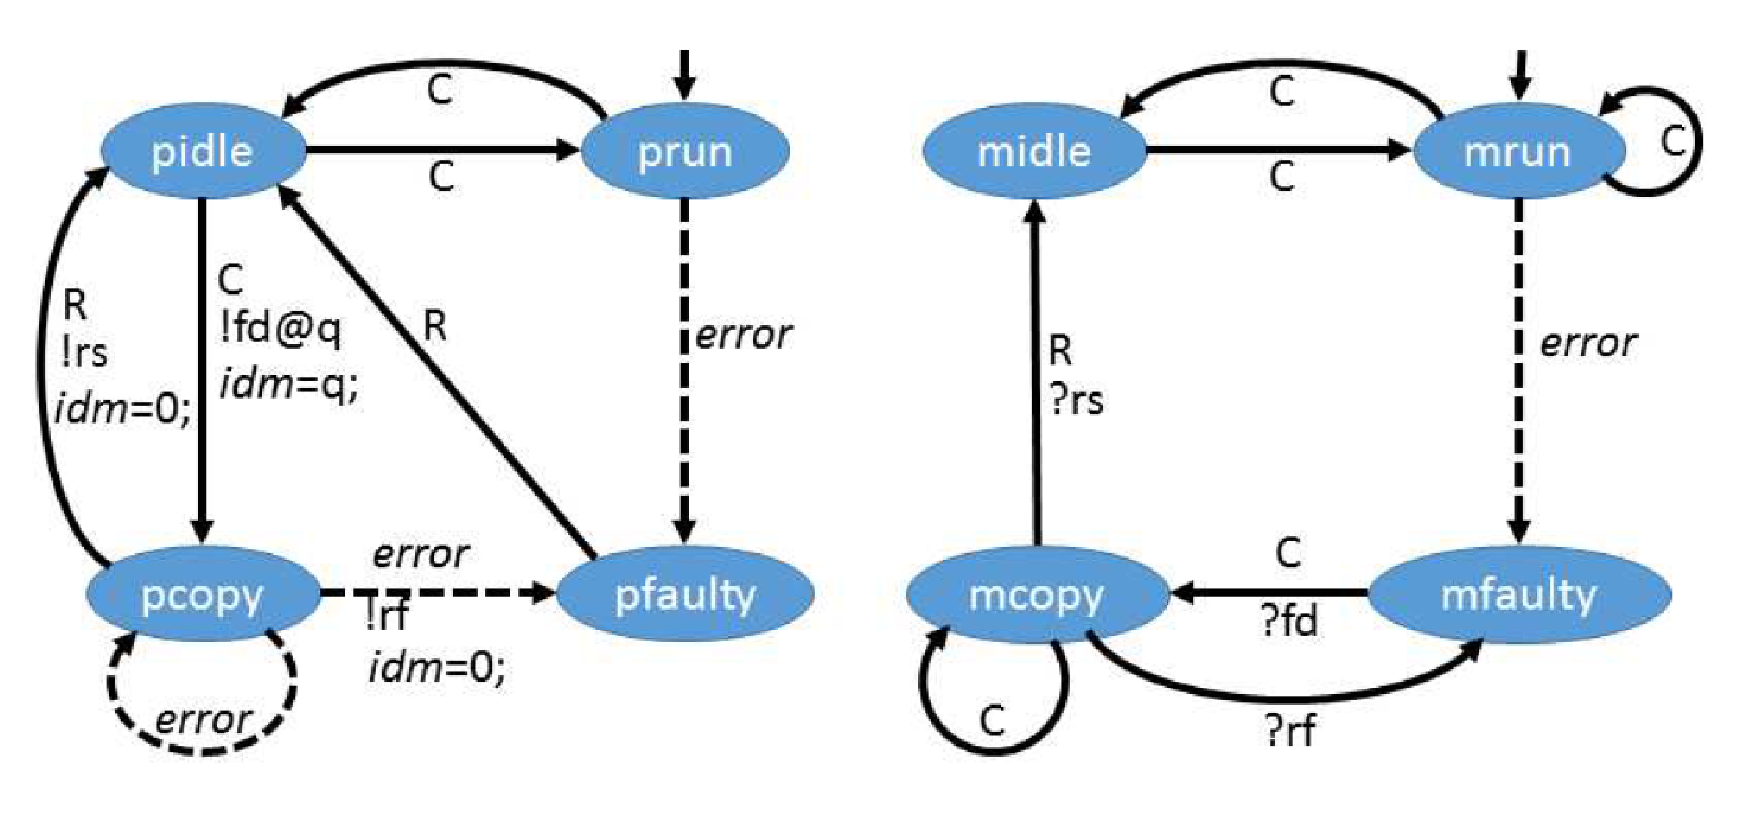
\epsfig{file=avi.eps,width=140mm} 
\caption{CEFSM templates of $n$ processors and $m$ memory copies}
\label{fig.pm}
\end{center} 
\end{figure*}
The CEFSM model has $n$ processors and $m$ memory modules. 
Figures~\ref{fig.pm}(a) and (b) are 
for the abstraction of processors and memory copies, respectively.  
The ovals represent local states of a processor or a 
memory module, while the arrows represent transitions. 
The transitions of a CEFSM are labeled with `$\emerr$', 
`C' (for Control), or `R' (for recovery).  

We also use synchronizers to bind process transitions. 
For example, when a memory module moves into a faulty state, 
an idle processor may issue an {\tt fd} (error-detected) event
and try to repair the module by copying memory contents from 
normal memory modules.  
Such error-detection is usually achieved with standard hardware.  
Note that the benchmarks are models that reflect the 
recovery mechanism, abstracting away the details of the original systems.  
A central issue in the design of this recovery mechanism is then 
the resilience level of the controlled systems.  
We need three synchronizers: 
\textit{fd} for error detection by a processor, 
\textit{rs} for recovery success, 
and \textit{rf} for recovery failure.  
The three synchronizers are used to bind a transition from a processor 
and another from a memory module into a synchronized transition.  
For example, a processor at state \textit{pidle} and 
a memory module at state 
\textit{mfaulty} may simultaneously enter their 
\textit{pcopy} and \textit{mcopy} states respectively
through synchronizers $!$\textit{fd} (for sending the synchronizer) 
and $?$\textit{fd} (for receiving). 
We also conveniently use a variable $q$ in this synchronized 
transition to capture the identifier of the memory module receiving 
the synchronizer.  
A transition without synchronization labels is considered a trivial 
synchronized transition.  
The transition system of the CEFSM operates with interleaving semantics 
at the abstraction level of the synchronized transitions. 

For counter abstraction, we need four global variables \textit{crp}, \textit{cfp}, 
\textit{crm}, and \textit{cfm} respectively 
to keep track of the numbers of running processors, faulty processors, 
running memory modules, and faulty memory modules. 
We also need a local variable \textit{idm} for each processor to record 
the faulty memory module identifier that the processor is 
responsible for recovery. 
We label the controllable, error, and recovery 
transitions respectively with `C', `$\emerr$', and `R'. 
We also label each transition with synchronizers and actions.  
At any moment, the processors and the memory modules 
may enter their running states, execute a task, and generate 
the outcome. 
A processor starts its execution from state \textit{prun} while 
a memory module starts from state \textit{mrun}. 


\subsection*{Step 2: building the product automata}
The product automata is a Kripke structure whose 
states are of is a vector $[p_1,\ldots,p_n,i_1,\ldots,i_n,s_1,\ldots,s_m]$ 
of $2n+m$ elements.  
For all $k$, $p_k$ and $i_k$ respectively represent the 
current location and the current \textit{idm} value of processor $k$ while 
$s_k$ represents the current location of memory module $k$.  
Then interleaving semantics that each time only a global transition 
(a single local process transition without synchronizers 
or two local process transition bound by a synchronizer) is executed 
is adopted to determine the transition relation from one state to another. 
Such techniques are standard in model construction.  
REDLIB can help in this regard by constructing the Kripke structure in 
an on-the-fly style to avoid the construction of those states not reachable 
from the initial state. 

\subsection*{Step 3: the labeling of the move vectors} 
After the second step, we have the game structure ready except for the 
move vectors on the transitions. 
We use $E_1=\{C,R,\mbox{\em nop}\}$, where {\em nop} represents ``no operation,"
and $E_2=\{\emnerr,\emerr\}$.  
Then we use the following three rules to label move vectors. 
\begin{list1} 
\item Every global transition with one component local process transition labeled 
	with $\emerr$ is labed with move vector $[\mbox{\em nop},\emerr\}$.  
\item Every global transition with a component local process transition labeled 
	with $R$ 	
	is labeled with move vector $[R,\emnerr]$.  
\item All other global transitions are labeled with move vector $[C,\emnerr]$.  
\end{list1} 


\subsection*{Counter abstraction of the example} 
We also use the CEFSM in figure~\ref{fig.pm} to explain counter abstraction. 
We need eight counter variables: 
{\em pr}, 
{\em pi}, 
{\em pc}, 
{\em pf}, 
{\em mr}, 
{\em mi}, 
{\em mc}, and 
{\em mf} to respectively record the 
number of processes in location prun, pidle, pcopy, pfaulty, mrun, midle, mcopy, and mfaulty
in a state.  
Then the counter abstraction of the CEFSM is in Figure~\ref{fig.pmC}.  
\begin{figure*}[t] 
\begin{center} 
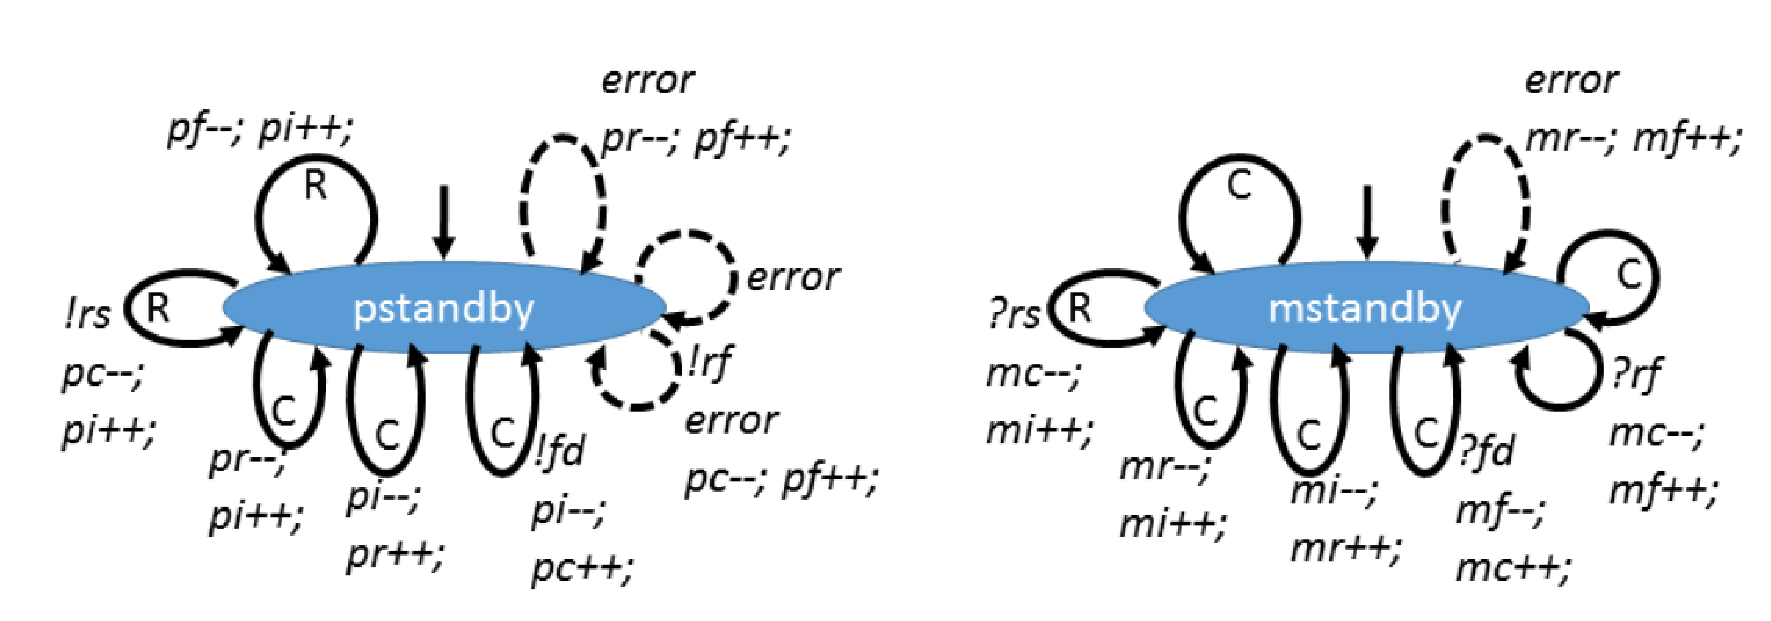
\epsfig{file=aviC.eps,width=140mm} 
\caption{Counter abstraction of the CEFSM templates of $n$ processors and $m$ memory copies}
\label{fig.pmC}
\end{center} 
\end{figure*}
The initial state are specified with constraint: 
$\mbox{\em pr}=n
\wedge \mbox{\em pi}=0
\wedge \mbox{\em pc}=0
\wedge \mbox{\em pf}=0
\wedge \mbox{\em mr}=m
\wedge \mbox{\em mi}=0
\wedge \mbox{\em mc}=0
\wedge \mbox{\em mf}=0$
on the counters.  
The state in the product automata must satisfy the following constraints: 
$\mbox{\em pr}+\mbox{\em pi}+\mbox{\em pc}+\mbox{\em pf}=n
\wedge \mbox{\em mr}+\mbox{\em mi}+\mbox{\em mc}+\mbox{\em mf}=m$.  
As can be seen, we do not care which processor is in the idle mode, 
in the running mode, etc., in this abstraction. 
Similarly, we do not care which memory module is in the idle mode, in the running mode, and etc. 
The local state transition only keeps tracks of the number of processors in each mode and 
the number of memory modules in each mode. 
We also do not care which processor is in charge of the recovery of which memory module.  
Such an abstraction can be done automatically.  

The labeling of the move vectors on the transitions in the Kripke structure (product automaton)
follows the same rules for the product automaton from the CEFSM in Figure~\ref{fig.pm}.  




\subsection*{Analysis of the game structure} 
The majority outcome of the processors and memory copies 
is used as the outcome of the system.  
A processor may enter the faulty state.  
A memory module may also enter the faulty state. 
Processors may control to recover themselves or a faulty memory module 
by copying the contents of a functioning memory module to 
the faulty one.  
At any moment, we want to make sure that we can always recover 
to a global condition with the following two restrictions. 
\begin{itemize} 
\item There are at least two more processors in \label{reply2.2more} 
	the running mode than the processors in the faulty mode.  
\item There are at least two more memory copies in 
	the running mode than memory copies in the faulty mode. 
\end{itemize} 
Together, the failure condition is 
$\textit{crp}-\textit{cfp}<2\vee\textit{crm}-\textit{cfm}<2$.  
That is, all states in the transition system satisfying 
$\textit{crp}-\textit{cfp}<2\vee\textit{crm}-\textit{cfm}<2$ 
are in set $F$.  

Tool implementation and the benchmarks used in the experiment 
can all be found in our Sourceforge REDLIB project at 
\verb+https://github.com/yyergg/Resil+.  






%
% The majority outcome of the processors and memory copies 
% is used as the outcome of the system.  
% A processor may enter the faulty state.  
% A memory module may also enter the faulty state. 
% Processors may control to recover themselves or a faulty memory module 
% by copying the contents of a functioning memory module to 
% the faulty one.  
% At any moment, we want to make sure that we can always recover 
% to a global condition with the following two restrictions. 
% \begin{itemize} 
% \item At least two more processors are in 
% 	their running states than in the faulty states
% \item At least two more memory copies are in 
% 	their running states than in the faulty states. 
% \end{itemize} 
%
\smallskip



\subsection{Performance data \label{subsec.exp}} 
% \noindent{\bf Performance data.}

We report the performance data 
in Table~\ref{tab.perf} for the resilience algorithms 
described in Section~\ref{subsec.bench} 
against the parameterized benchmarks in the above with various 
parameters.  
The second column shows the concurrency sizes.  
The third column shows the values of $k$ for the rows.  
The fourth and fifth columns show the sizes of the concurrent game structures.  
The sixth and seventh columns show the time and spaces used to calculate 
sfrch$_k()$.  
Similarly, the eighth and ninth columns show the time and spaces for calculating 
the res$_k()$.  

The benchmark in Figure~\ref{fig.pm} does not have nodes in 
$\safe_2(G)$ and $\res_2(G)$.  
So we changed the benchmark to see how we check our implementation 
with $k>1$.  
The change is that the recovery transition from state \textit{pcopy} to 
\textit{pidle}
of processors are relabeled as controllable. 
This change significantly limits the ability of the system errors 
to derail the system.  
\begin{table*}[t] 
\caption{Performance data for resilience calculation \hspace{21mm} s: seconds; M: megabytes} 
\label{tab.perf} 
\begin{center} 
\begin{tabular}{l|c|c|c|c||c|c||c|c} \hline 
benchmarks & concurrency & $k$ & \multicolumn{2}{c||}{game sizes} 
& \multicolumn{2}{c||}{sfrch$_k$}  
			& \multicolumn{2}{c}{res$_k$} \\\cline{4-9} 
	 & 	& & \#nodes & \#edges & time  & memory   & time & memory  \\
\hline \hline 
avionics & 2 processors \& 2 memory modules 
     & 2 & 118 & 750 
     & 0.62s & 114M & 0.85s & 116M \\ \cline{2-9} 
     & 2 processors \& 3 memory modules 
     & 2 & 414 & 3252
     & 0.94s & 139M & 1.10s & 153M \\ \cline{2-9} 
     & 3 processors \& 3 memory modules 
     & 3 & 1540 & 15090 
     & 4.67s & 225M & 8.38s & 267M \\ \cline{2-9} 
     & 3 processors \& 4 memory mdules
     & 3 & 5601 & 63889 
     & 42.86s & 815M & 155s & 846M \\ \hline  
avionics & 6 processors \& 6 memory modules 
	 & 2 & 1372 & 6594 
	 & 2.89s & 129M & 3.54s & 516M \\ \cline{2-9} 
(counter	 & 7 processors \& 7 memory modules 
	 & 3 & 2304 & 11396 
	 & 10.7s & 216M & 23.4s & 808M \\ \cline{2-9}
abstraction)	 & 8 processors \& 8 memory modules 
	 & 3 & 3645 & 18432 
	 & 43.8s & 1009M & 135s & 2430M \\ \hline 
voting	 & 1 client \& 20 replicas 
	 & 9 & 9922 & 23551 & 7.01s & 260M & 36.7s & 297M \\ \cline{2-9} 
	 & 1 client \& 26 replicas 
	 & 12 & 20776 & 49882 & 19.9s & 474M & 79.6s & 611M \\ \hline 
simple	 & 1 client \& 150 replicas 
	 & 74 & 458 & 1056 & 0.71s & 159M & 31.7s & 219M \\ \cline{2-9} 
voting	 & 1 client \& 200 replicas 
	 & 99 & 608 & 1406 & 1.06s & 161M & 162s & 337M \\ \cline{2-9} 
	 & 1 client \& 250 replicas 
	 & 124 & 758 & 1756 & 1.36s & 163M & 307s & 499M \\ \hline 
PBFT 	 & 1 client \& 6 replicas 
	 & 2 & 577 & 897 & 0.34s & 72M & 1.05s & 193M \\ \cline{2-9} 
	 & 1 client \& 9 replicas 
	 & 4 & 2817 & 4609 & 13.3s & 564M & 58.5s & 1657M \\ \hline 
clock	 & 1 client \& 15 servers  
	 & 7 & 16384 & 229376 & 45.1s & 3075M & 62.4s & 3264M  \\ \cline{2-9} 
sync	 & 1 client \& 17 severs  
	 & 8 & 65536 & 1070421 & 870s & 14725M & 915s & 15433M  \\ \hline 
\end{tabular}
\end{center}
\vspace*{-5mm}
\end{table*}
For the avionics system, %the $k$ value
the resilience level $k$ is set to 
one less than half the %value
number of processors.  
For the voting and simple voting benchmarks, 
the value of $k$ is set to one less than half the number of 
replicas (voters). 
For the PBFT and clock synchronization algorithm, we choose 
$k$ to be one less than one third of the number of replicas. 

The performance data has been collected with a Virtual Machine (VM) 
running opensuse 11.4 x86 
on Intel i7 2600k 3.8GHz CPU 
with 4 cores and 8G memory. 
The VM only uses one core and 4G memory.  

The time and space used to calculate resilience is a little bit more 
than that to check for $\safe$.  
The reason is that $\safe_k$ is a pre-requisite for calculating $\res_k$.  
In our experiment, $\safe_k$ is usually 
very close to $\res_k$ and does not require much extra time in 
calculating $\res_k$ out of $\safe_k$.  

The experiments show that our techniques 
scale to realistic levels of redundancy.  
For fault-tolerant hardware, usually the numbers of replicas are small, 
for example, less than 10 replicas. 
Thus our techniques seem very promising for the 
verification and synthesis\label{reply2.verification.hardware} of hardware fault-tolerance.  

On the other hand, 
nowadays, software fault-tolerance through networked computers can 
create huge numbers of replicas.  
Our experiment shows that counter abstraction can be a useful 
techniques for the modeling and verification of software resilience.  
Specifically, for the avionics benchmark, 
we can verify models of much higher concurrency and complexity with 
counter abstraction than without. 
% As can be seen, our techniques can really prove the % safety and 
% resilience of pretty large concurrency sizes.  





\section{Related work\label{sec.relwork}}

We have applied game-based technqiues~\cite{Church63,PR89a,Rabin69} \label{reply1.related.work.1st.para} 
for synthesizing a control mechanism with maximal resilience to software errors.  
The synthesis of control strategies is essential in solving games with temporal and $\omega$-regular objectives.  
For these more complex objective, synthesis goes back to Church's solvability problem~\cite{Church63} and 
inspired Rabin's work on finite automata over infinite 
structures~\cite{Rabin69} and 
B\"uchi and Landweber's works on finite games 
of infinite duration~\cite{Buchi62,BL69}. 
A righ body of literature on synthesis
has since been developed \cite{AAE04,EKA08,GR09,KV00,PR89b,Rushby92,SF06}.

Traditionally, fault tolerance refers to various basic fault models~\cite{AAE04}, 
such as a limited number of errors \cite{JRT04}.
These traditional fault models are subsumed 
by more general synthesis or control objectives 
\cite{AMP95,AAE04,Thomas94};\label{reply2.RW} 
as simple objectives with practical relevance, 
they have triggered the development of specialized tools~\cite{EKA08,GR09}.

Dijkstra's self-stabilization criterion~\cite{AG93,Dijkstra86} suggests to build systems that eventually recover
to a `good state', from where the program commences normally.
Instead of {\em constructing} a system to satisfy such a goal, one
might want to apply control theory to {\em restrict} the execution of
an existing system to achieve an additional goal.
Our control objective is a recovery mechanism for up to $k$ errors.
After recovery, the system has to tolerate up to $k$ errors again, and so forth.
In this work, 
we suggest a mechanism to synthesize a recovery mechanism for a given fault model and recovery primitives.


In \cite{DHLN10}, an interesting notion of robustness based on Hamming 
and Lewenstein distance related to the number of past states is defined. 
It establishes a connection between these distances with a notion of 
synchronization that characterizes the ability of the system to reset for 
combinatorial systems.
In \cite{BGHJ09}, `ratio games' are discussed, where the objective is 
to minimize the ratio between failures induced by the environment and system errors caused by them.


Besides using our simple game model that neither refer directly to time, nor to probabilities, one can also consider models that make these aspects explicit.
Their analysis is far more complex (with \cite{FRSZ11} offering the best complexity bounds), and so are the resulting strategies.
If we, for example, return to the example of airplanes with an operation time of 20 hours referred to in Table \ref{tab.mtbf}, then an optimal timed model would take the remaining operation time into account.
When the remaining time is two minutes, the balance between being resilient against waves of two errors and being resilient against 5 errors looks very different, and the optimal control would change over time rather than being static.
Another implication of more complex models would be that the error model would have to be more detailed.
Even if one assumes that a simple concept like safe states persists, it depends on the fineties of such a model if a two step path back to it where an error after step one leads to system failure is preferable over a much longer path, say through 10,000 intermediate states, where one error can be tolerated during recovery.

We believe that the independence from such details is an advantage of our technique, partly because it is simpler and cheaper, and partly because the further advantages one can obtain from more detailed error models rely heavily on very knowledge of (or, realistically, on very detailde assumptions on) how errors are distributed.
\label{reply1.prob.more.complex}  

%\paragraph{\bf Organization of the article.}
%We suggest a two layered approach:
%in a first layer, we simplify a complex system to the aspects relevant for its control.
%This abstraction layer of our approach reduces life size examples to small abstractions 
% (Example~\ref{exmp.avi}).
%%
%In Section~\ref{sec:kresil}, we provide computationally cheap algorithms to synthesize a strategy for controlling the system to allow for up to $k$ dense failures.
%Such a strategy restricts the choices of the system to achieve resilience towards $k$ failures.
%Failure to construct such a strategy means that the system is not $k$-resilient.
%% Through the abstraction used, a
%Achieving the fault tolerance goal by controlling the system through the calculated strategy, provides a guarantee that the executions of the controlled system are included in the original executions of the system.
%This, in turn, guarantees that {\em all} (linear) temporal properties of the system are preserved.
%%
%We describe our implementation and discuss experimental results in Section~\ref{sec.imp.exp}.

%% >>> changes start 


In \cite{EhlersT14,BloemEJK14} the resilience model we have introduced \cite{HPSW/12/rapidRecovery} has been applied for synthesising robust control in an assume-guaranee setting to produce robustness against occasional noncompliance of the environment with the assumptions of its behavior.

%% <<< changes end

\section{Conclusion \label{sec.conc}}
We have introduced an approach for the development of a control of safety critical
systems that maximizes the number of \emph{dense} errors the system can tolerate.
Our techniques are inspired by the problem of controlling systems with redundancy:
in order to deflect the effect of individual errors, safety critical systems are often equipped with multiple copies of various components.
If one or more components fail, such systems can still work properly as long as the correct behavior can be identified.
 
This has inspired the two-phase formulation of the safety resilience problems in this article.
In the first phase, we identify a $k$-resilient region\label{reply2.need.identify},  
while\label{reply2.layer} we develop a control strategy for recovery in the second phase.  
After an error, the controller can recover to the $k$-resilient region without encountering a system failure, unless the error is part of a group of more than $k$ errors that happen in close succession.
Such a recovering strategy is memoryless.
Being memoryless on a small abstraction in particular implies that the recovery is fast.

The system can, once recovered, tolerate and recover from $k$ further dense errors, and so forth.
Consequently, our control strategy allows for recovery from an arbitrary
number of errors, provided that the number of dense errors is restricted.
This is the best guarantee we can hope for: our technique guarantees to find the optimal parameter $k$.
%
This parameter is bound to be small (smaller than the number of redundant components).
Optimizing it is computationally inexpensive, but provides strong guarantees: the likelihood of having more than $k$ errors appear in short succession after an error occurred are, for independent errors, exponential in $k$. As errors are few and far between, each level of resilience gained reduces the likelihood of 
system-level failures significantly.


   

\bibliographystyle{abbrv}
\bibliography{valcite.151008.sven}
% \bibliography{../../../valcite}




\newpage
\onecolumn 
\begingroup
\appendix 
\begin{center} 
\bf\LARGE The Second-round Revision \\
(Summary) 
\end{center} 
Dear editors,\\
dear reviewers: 

According to the reviewers' comments and suggestions, 
we have significantly reshaped the manuscript.  
We have addressed all the issues raised by the reviewers.  
The major changes are the following. 
\begin{list1} 
\item Reviewer 1 pointed out that there could be a confusion between 
    evaluation and controller synthesis in understanding the manuscript. 
    The concern is indeed very valid and 
    the presentation could create misunderstanding to readers of 
    various background. 
    As a result, we have decided to change the presentation a little bit toward 
    controller synthesis.  
    Thus, the title of the manuscript has been again changed from 
	\begin{center} \em 
	A Formal Foundation for the Quantitative Evaluation of Software Resilience against Dense Errors.
	\end{center} 
	to 
	\begin{center} \em 
	A Game-Theoretic Foundation for the Maximum Software Resilience against Dense Errors.
	\end{center} 
	Many parts of the manuscript have also undergone revision in this line. 
\item We have rewritten the definition of AMCE for readability. 
    We now begin Section~\ref{sec.amc} with several small examples. 
    The syntax and semantics presentation of AMCE are also changed 
	to better follow the style of \cite{AHK02}. 
	As a result, the syntax and semantics are simplified and, 
	in our opinion, easier to understand.  
\item We have also corrected glitches in the presentation, 
    including several typos and providing the url to the experiment material,
\begin{center}
\verb+https://github.com/yyergg/Resil+
\end{center} 
\end{list1} 
In the following, we provide the detailed revision report to the reviewers.  
We hope that the reviewers will be satisfied with the revision.  
If there is any question, please do not hesitate to let us know. 

\newpage 
\begin{center} 
\bf\LARGE The Second-round Revision Summary 
\end{center} 
\section{Responses to the editor} 

\begin{verbatim} 
**************
Editor Comments

Editor
Comments to the Author:
The major technical concerns of the reviewers with the previous paper largely 
have been addressed in the new submission.  
However, there are some significant weaknesses in terms of the clarity of the 
descriptions that make it not appropriate for TSE publication.  
Both reviewers note places in the presentation that are not described 
well enough to be understood.  
Please consider their comments regarding sections and sentences that 
caused confusion or that appeared to be incorrect, and revise accordingly.   
Please also ensure that the url for accessing your implementation 
and benchmarks is correct. (Like Reviewer 1, I could not find them.)
\end{verbatim} 
\begin{reply0} 
Thanks for the comments and suggestions.  
Thank you in particular for pointing out the missing link. 
In this revision, we have tried to address all issues raised by the 
reviewers, including the following url for the experiment materials. 
\begin{center}
\verb+https://github.com/yyergg/Resil+
\end{center} 
\end{reply0} 
\begin{verbatim} 
********************
Reviewers' Comments

Please note that some reviewers may have included additional comments 
in a separate file. 
If a review contains the note "see the attached file" 
under Section III A - Public Comments, you will need to log on 
to ScholarOne Manuscripts  to view the file. 
After logging in, select the Author Center, click on the 
"Manuscripts with Decisions" queue and then clicking 
on the "view decision letter" link for this manuscript. 
You must scroll down to the very bottom of the letter to see the file(s), if any.  
This will open the file that the reviewer(s) or the Associate Editor 
included for you along with their review.

\end{verbatim} 





\newpage 
\begin{center} 
\bf\LARGE The Second-round Revsion Report 
\end{center} 
\section{Responses to the 1st reviewer} 

\begin{verbatim} 
Reviewer: 1

Recommendation: Author Should Prepare A Major Revision For A Second Review

Comments:
The paper 
"A formal Foundation for the Quantitative Evaluation of Software Resilience 
against Dense Errors"
deals with the question how error-resilient a (software) system is. 
The authors propose finite-state games as computational model and advocate 
that the notion of k-resilience is the right one to study the error-resilience 
of a system. 
If a system is k-resilient, this means that it can tolerate infinitely many 
sequences of up to k errors each, provided that in between these sequences, 
there is enough time for the system to recover.

Apart from checking a given system for k-resilience, the authors also show 
how to control a system to be k-resilient for an as high number of k as possible. 
They derive a formula in alternating mu-calculus that only needs to 
be evaluated in order to find a strategy to control the system that achieves this.
The algorithm runs in PTIME, and the authors prove that the problem 
is also PTIME-hard.

The study of error-resilient systems is interesting and the paper shows 
that their design can be automated to some extent by algorithms 
with a low complexity. 
Yet, the paper is not ready to be published in its current form. 
The presentation is confusing at some 
places and the concepts presented are not structured in a clear way. 
This makes reading the paper less pleasant than necessary, 
and given that the core results are not very 
complicated, not appropriate for the content of the paper. 

The confusion already starts in the abstract. 
It mixes evaluating the system's error 
resilience with controlling the system: 
first the authors state that they develop a 
framework for *evaluating* the defense strength of a software system, 
and then talk about resilience as a *control objective* in such a game. 
Then the abstract talks about the analysis of k-resilience problems 
with "model checking" written next to it - which 
suggests evaluation again, but then, the abstract talks about 
"optimal control strategies" again. 
So the focus seems to be a bit more on control, 
although the title of the paper talks about evaluation.
\end{verbatim} 
\begin{reply1} \label{reply1.eval.control} 
Thanks for the comments and suggestions.  
We are really sorry for the confusion caused. 
In fact, there are two aspects of this work. \\
(1) Evaluation of how strong a system can be in resilience in game's perspective. (I.e., when controlled optimally.) \\
(2) Synthesis of a control strategy to achieve the maximal resilience.  \\
In this perspective, the work is about both evaluation and control.  
However, we think that your concern is very valid.  
We thus changed the presentation toward control synthesis and implemented the 
following two changes. 
Firstly, we have changed the title again to the following. 
\begin{center} \bf 
A Game-Theoretic Foundation for the Maximum Software Resilience against Dense Errors.
\end{center} 
Secondly, we have added the following sentence to the abstract to increase clarity.
\begin{center} 
\parbox{140mm}{\em 
We propose a game-theoretic foundation for synthesizing control strategies 
that maximize the resilience of a software system in defense against a
realistic error model.  
}
\end{center} 
\end{reply1} 
\begin{verbatim} 
The beginning of the introduction clears the issue a bit 
- games are needed to evaluate the error-resilience of systems. 
The authors explicitly write that 
"a game-theoretic foundation for such a purpose" is built. 
Ok, so the "control" from earlier may have been 
referring to playing games, rather than actually controlling systems. 
But then later in the introduction, the focus seems to be on control 
in the sense of influencing a system's behavior again. 
This is highly confusing! 

The paper must be crystal clear on what is being achieved. 
If it is evaluation *and* control, 
this should be stated as such right from the start. 
At the moment, the reader is already confused before she comes to the point 
where the scope of the paper is explained. 
\end{verbatim} 
\begin{reply1} 
Thanks!
Hopefully the revision as described in reply 1.~\ref{reply1.eval.control} 
can make our manuscript clear in this regard. 
\end{reply1} 
\begin{verbatim} 
Furthermore, given that evaluation is a model checking problem, it does not 
become clear to the reader why a game is actually needed at all for this purpose. 
Resilience should be evaluatable on the trace/model checking level. 
The answer that I derived from the technical results of the paper is that 
the game is only needed because the duration of recovery is not known in advance, 
so declaring recovery to be done is the task of one of the players. 
Controlling a system can then be added as an additional winning criterion 
in the game.
\end{verbatim} 
\begin{reply1} 
Thanks for the argument.  
The game concept is employed in this work since there could be many measures 
to control the system and the designers want to find out the best way 
to use the measures to achieve maximal resilience.  
For example, when a request is not responded to by the system, 
we may redo the request, or we may reset the system, or clear some communication 
buffer.  
But in general, the system designers may need support in finding out the 
best solution.  
That is how game concept comes in.  
In fact, we follow the classic work by Pnueli and Rosner \cite{PR89a,PR89b} 
in using finite-transition system models for the research of the synthesis problem 
of control strategies.  
To clarify the issue, we have added the following sentences to the first 
paragraph of the introduction. 
\begin{center}
\parbox{140mm}{\em 
Programmers 
and software designers have developed many engineering 
techniques to contain the damage that could be caused by such defects.  
For example, when observing that a critical service request is not 
acknowledged, a software system may have several measures to its disposal to
avoid system failure, including 
resending the request, 
resetting the server, 
clearing the communication buffers, etc. 
But, in general, it is difficult to estimate how to organize the measures 
for the maximal resilience of the system against realistic errors.  
At the moment, an automated support for the synthesis of 
control mechanism to defend a system against software errors is missing.  
Such an automated support, if available, can suggest defense techniques against software defects to development teams,
and help these development teams to identify the vulnerabilities of software systems.    
We use a game-theoretic approach to study this aspect and have
carried out experiments to 
observe how our techniques can be used in synthesizing the most resilient 
defense of software systems against multiple errors.  
}
\end{center} 
Please check page~\pageref{reply1.control.eval.intro}.  
\end{reply1} 
\begin{verbatim} 
The paper is also confusing in a few other ways. 
For example, why is it actually necessary to define safe states at all? 
During the evaluation of resilience, they should not be needed. 
Also when controlling the system, there should be no need to give them explicitly. 
And later, control is actually done without this state set being known 
beforehand, with the motivation that asking the user to provide these 
is error-prone. 
So the only reason to introduce them in the first place is because 
the safe states take a central role in all of the definitions, 
and so it is not clear if the whole approach makes sense 
without them having been defined in advance. 
Basing the definitions on an artifact that is computed in the process 
is very non-straight-forward and should be avoided whenever possible. 
The problem here seems to be that the authors avoid to 
define the allowed length of a recovery period as a parameter to k-resilience. 
This would allow to clean up the definitions and allow them to state that 
what they actually search for is the highest value k such that 
exists a recovery period length such that all periods are below this length. 
All other definitions could then be made without referring to safe states. 
As a side effect, this would also allow the authors to get rid of the rather 
nebulous remarks about how memorylessness of strategies helps with ensuring 
that such a bound exists - 
it is much more convincing if memorylessness of optimal strategies 
follows from the analysis of the game.
\end{verbatim} 
\begin{reply1} 
Thanks for the comments and suggestions.  
We apologize if we did not make the idea clearer.  
The identification of safe states is central to our proposal for 
resilience to repetitive waves of software errors without bounding the 
time for recovery.  
All our algorithm is then developed according to this concept.  
As we mentioned in the introduction, there are three cases to use our tool 
and techniques.  
The first case is to check whether a given safe state set is good for 
$k$-reslience while the other two cases do not require the users to 
provide the input of safe state.  
Your concern that the safe state set prescribed by the users could be erroneous 
only can happen in the first case.  
Still, in the first case, our tool can then check whether the 
user-prescribed set of safe states is good for $k$-reslience.  
The users do not have to worry about whether they may build a software 
system based on false resilience assumption.  
That is what we want to do in this work: to provide automated support for 
designing systems with maximal resilience.  
We would like to assure you that whether the user is error-prone in prescribing 
safe state set should not be a concern to our approach since our tool is designed 
to help detecting and removing such errors.  
The user has to specify, what should not happen (failures), and what the events that can harm the system are (errors), while the approach we develop has the task to find the optimal defence against against failure (i.e., a strategy that offers the maximal resilience level).

Indeed, your comments and suggestions are valuable and may lead to 
other solutions and algorithms for resilience control.  
However, we feel that, at the moment, it is better and more practical to 
leave your suggestions for future work.  
\end{reply1} 
\begin{verbatim} 
All in all, I think that the presentation can be improved substantially. 
Even if the reformulation of the definitions is refused by the authors, 
the following further remarks provide more reasons why I believe 
that this assessment is fair. 
\end{verbatim}
\begin{reply1} 
Thanks for the suggestions. 
We hope that our revision and replies respond to your concerns well. 
If there is any question, please do not hesitate to let us know. 
\end{reply1} 
\begin{verbatim}
- In the footnote on the first page, something called "tgg" is mentioned. 
However, it is not clear at this point what is meant. 
\end{verbatim}
\begin{reply1} 
Thanks for the corrections. 
``tgg" is the name used for our tool implemented for this work. 
We have removed the name from the footnote and updated the webpage address. 
Please check page~\pageref{reply1.tgg}. 
\end{reply1} 
\begin{verbatim}
- Page 2, column 1, lines 31-38: these sentences of prose seem to be redundant
\end{verbatim}
\begin{reply1} 
Thanks for the comments. 
We feel that if we are to follow your previoius suggestion to make an assumption 
on the duration length of recovery segments, then these two sentences 
are indeed redundant. 
But if we want to propose a theoretical foundation that 
allows for the analysis and synthesis of resilient control mechanism 
that can endure software errors without any assumption on the duration of 
recovery segments, then these two sentences are helpful in motivating the 
readers to continue their reading of the work. 
So, we would like to ask for your understanding of our decision to keep these 
two sentences.  
\end{reply1} 
\begin{verbatim}
- Page 2, column 1, lines 38-43: system failure is later defined to be the 
incorrect behavior of a system. 
However, here it is stated that the system fails 
if an incorrect error model is used. 
But the error model itself is not part of the system's implementation, 
but rather a modelling and analysis artifact, 
so how can it be that a system fails if we model 
its environment incorrectly? 
Note that at this point of the paper, the authors still talk 
about the analysis of an already existing system. 
I guess that this paragraph is another example of the authors jumping back 
and forth between analysis and control without 
distinguishing these objectives properly.
\end{verbatim}
\begin{reply1} 
Thanks for the comments. 
Indeed in this paragraph, we had confused model analysis with system runtime behavior.
We have changed the troubled sentences to the following. 
\begin{center} 
\parbox{140mm}{\em 
Apparently, no non-trivial system can endure an unlimited flood of errors without 
degrading to inevitable system failure. 
Thus, if we do not employ a realistic error model, then 
no meaningful analysis of the resilience level of these systems to software errors can proceed, 
and no practical control mechanism can be devised to defend them against errors.   
}
\end{center} 
Please check page~\pageref{reply1.realistic.system.failure}.  
\end{reply1} 
\begin{verbatim}
- Page 2, column 2, lines 1-9: this sentence needs to be rewritten. 
Right now, a system that recovers to "safe behavior" immediately 
would be less error resilient than one that takes longer to do so, 
as it could endure fewer error before recovery to safe behavior. 
\end{verbatim}
\begin{reply1} 
Thanks for the comments. 
Indeed your concern is valid if the system model in unconstrained. 
But in our system models of finite-state graphs, the number of errors that 
can be injected is also restricted by the structure of the model.  
Thus, the definition that concerns you should not be an issue if the 
protagonist uses a strategy to restrict the domain of plays.  

Also, we have changed the sentence to the following to better clarify our 
contribution. 
\begin{center} 
\parbox{140mm}{\em 
In this work, we propose to evaluate control mechanism 
of software systems on 
how many errors the control can endure before recovery to safe behavior. 
We then present an algorithm to synthesize a control strategy
that can endure the maximal number of such errors.  
}
\end{center} 
Please check page~\pageref{reply1.less.errors.more.resilient}.  
\end{reply1} 
\begin{verbatim}
Also, wouldn't it be appropriate to say that the recovery behavior 
is "safe behavior" as well? 
In a sense, it is even safer than the regular operation of the system.
\end{verbatim}
\begin{reply1} 
Thanks for the comments. 
But we think the opinion that a system is safer in the recovery segment is really subjective. 
Depending on the technology, 
in system recovery, the control mechanism may reboot the software, 
flush the caches, or even update protected data in critical section.  
Defense against failures in recovery segments is a difficult and challenging 
research issue in operating systems and programming languages. 
\end{reply1} 
\begin{verbatim}
- Page 2, column 2, lines 37-40: this sentence is grammatically incorrect
\end{verbatim}
\begin{reply1} 
Thanks for pointing this out. 
Since we have changed the presentation focus to control synthesis, we 
use the following sentence to replace the sentence that you mentioned. 
\begin{center} 
\parbox{140mm}{\em 
Our specific goal is to develop a technique for synthesizing a 
control mechanism of a software system against the maximal number of dense errors 
without degrading to failure.
}
\end{center} 
Please check page~\pageref{reply1.grammar.inco.specific.goal}. 
\end{reply1} 
\begin{verbatim} 
- Table 1: The caption says "mean time between dense errors", 
but the table does not contain any times.
\end{verbatim}
\begin{reply1} 
Thanks for pointing this out. 
We have changed the caption to: {\em Probabilities of $k$ dense errors}.  
Please check page~\pageref{tab.mtbf}. 
\end{reply1} 
\begin{verbatim} 
- In general, Having "player 1", "protagonist", *and* "system player" 
as names for the same player is too much. 
Also, the player roles are motivated several times, which 
always makes the reader wonder if something new is coming next or not.
\end{verbatim}
\begin{reply1} 
Thanks for pointing this out. 
We have moved the comments on the terms to the footnotes and 
then used protagonist (antagonist) to replace 
player 1 (respectively player 2) throughout the manuscript. 
Please check page~\pageref{reply1.protagonist.player1}. 
\end{reply1} 
\begin{verbatim} 
- Page 3, column 2, line 43: at this point, 
it is not clear why this is a game at all, 
as only one player seems to be able to make non-trivial moves. 
In line 45, it is then stated that the "protagonist plays by selecting a move, 
intuitively the normal event that should happen next". 
Apart from the grammar error, if we are analyzing an existing system, 
why is there a choice at all? If the non-determinism comes from the abstraction,
then in order not to over-estimate the value of k, 
this choice should be up to the antagonist, and not up to player 1.
\end{verbatim}
\begin{reply1} \label{reply1m.abstraction}
Thanks for your question. 
Following your suggestions, we have 
now revised the manuscript toward controller synthesis research.  
In such a framework, the choice of the protagonist does not come from 
abstraction.  
Intead, the protagonist (the system) may have several measures to control 
the scenaior and plays and defend itself against the errors. 
As we have now explained in the introduction, 
the designers may not know what is the best way of using the measures.  
Thus our work is for developing techniques to automatically synthesize a 
strategy of using the measures.  

Also, the faiulre mode in our model can indeed inject errors 
which is also supposedly nontrivial. 
Thus the roll-out of the plays is not completely determined by the protagonist. 
\end{reply1} 
\begin{verbatim}
- Page 4, line 7: "memoryless" - it is too early to rely on this. 
Memorylessness of strategies should follow from the winning condition 
in your games, and not be assumed a-priori.
\end{verbatim}
\begin{reply1} 
Thanks for your suggestion. 
Yes, indeed, our result are obtained without assuming memoryless strategies.  
In fact, this sentence is a comment about what we are to prove in the manuscript. 
We decide to make the statement about memoryless strategies in future tense.  
In that way, the readers can understand this is a comment about what we 
are to prove.
Please check page~\pageref{reply1.memoryless.future}.  
\end{reply1} 
\begin{verbatim}
- Page 5, column 1, line 20: "participated by multiple players"
\end{verbatim}
\begin{reply1} 
We have changed the sentence to the following. 
\begin{center} 
\parbox{140mm}{\em 
A concurrent game may involve several players, 
who make concurrent move decisions at the same time during transitions. 
}
\end{center} 
Please check page~\pageref{reply1.multiple.players}.  
\end{reply1} 
\begin{verbatim}
- Page 5, column 1, line 45: Why is "r" used as initial state? 
This choice is very uncommon. 
"q_0" or "q_start" are much more common.
\end{verbatim}
\begin{reply1} 
Sorry for the notations. 
$r$ stands for ``root."
We also used $q_0$ in some previous papers.
But when we discuss plays as functions from 
natural numbers to states and move vectors, it is convenient to introduce subscripts to the states (and move vectors) in the plays. 
In that situation, it becomes cumbersome to deal with the subscripts of the 
initial states.  
\end{reply1} 
\begin{verbatim}
- Page 5, column 2, line 7-8: 
"For convenience, we require that every state has a successor state" 
- Why for convenience? \delta is defined to be a total function from Q 
\times E_1 \times E_2 to Q, so of course every state has a successor state
\end{verbatim}
\begin{reply1} 
Thanks for pointing this out. 
Thus we have removed the sentence.  
Please check page~\pageref{reply1.for.convenience.succ}.  
\end{reply1} 
\begin{verbatim}
- Page 5, column 2, line 21-25: grammar
\end{verbatim}
\begin{reply1} 
Thanks for pointing this out. 
We have moved the ``or" to the last phrase.  
Please check page~\pageref{reply1.grammar.or}.  
\end{reply1} 
\begin{verbatim}
- Page 6, column 1, line 28: 
"Given a strategy \sigma_a of player a for every a \in \{1,2\}" 
- the grammar needs to be fixed here. 
Either it is one strategy or two strategies. 
\end{verbatim} 
\begin{reply1} 
Thanks for the correction. 
We have rewritten the two sentences as follows. 
\begin{center}
\parbox{140mm}{\em 
Formally, a strategy $\sigma_a$ for a player $a\in\{1,2\}$ is a function from play prefixes to $E_a$.  
The next state after a play prefix $\rho\in \big(Q(E_1 \times E_2)\big)^*Q$ 
is determined as 
$\delta(\emlast(\rho),\sigma_1(\rho),\sigma_2(\rho))$. 
}
\end{center} 
Please check page~\pageref{reply1.grammar.strategy}.  
\end{reply1} 
\begin{verbatim} 
Also, in the next line, there seems to be a \times missing between Q and (E_1.
\end{verbatim} 
\begin{reply1} 
Sorry for the confusion about our notations. 
We thus introduced the following paragraph before definition~\ref{def.strategy} 
to explain our notations. 
\begin{center}\parbox{140mm}{\em 
We may also use regular expressions to represent sets of play prefixes.  
Specifically, given two sets $A$ and $B$ of play prefixes, 
$AB$ represents the set of concatenation of play prefixes $\rho_1\rho_2$ 
such that $\rho_1\in A$ and $\rho_2\in B$.  
$A^*$ then represents finite concatenation of play prefixes from $A$.  
For example, $a,abc,abcacbcbcbc$ are all elements of $\{a,bc,ac\}^*$.  
}  
\end{center} 
Please check page~\pageref{reply1.regexp.concat}.  
\end{reply1} 
\begin{verbatim} 
- Page 8, column 1, lines 43-49: the commas in lines 46-49 need to be removed
\end{verbatim} 
\begin{reply1} 
The two commas have been removed. 
Please check page~\pageref{reply1.cases.comma}.  
\end{reply1} 
\begin{verbatim} 
- Page 8, column 1, lines 50: inserting an "of this paper" 
after the reference [25] would clarify what it meant here.
\end{verbatim} 
\begin{reply1} 
Thanks for the suggestion. 
Phrase inserted accordingly. 
Please check page~\pageref{reply1.of.this.paper}.  
\end{reply1} 
\begin{verbatim} 
- Page 8, column 1, last few lines: 
here, it is stated again that the aim of this paper is to design a framework 
for *evaluating* system resilience, although earlier, the authors 
wrote about control.
\end{verbatim} 
\begin{reply1} 
Sorry for the confusion. 
We have changed the sentence to the following. 
\begin{center} 
\parbox{140mm}{\em 
In this work, we use these observations to design a theoretical framework for synthesizing a control mechanism that provides 
the maximal resilience against software errors in a realistic error model. 
} 
\end{center} 
Please check page~\pageref{reply1.theoretical.framework.eval}.  
\end{reply1} 
\begin{verbatim} 
- Page 8, column 2, lines 18-21: this sentence has multiple grammatical problems: 
it mixes singular with plural forms, 
and an "a" and a "the" is missing before "recovery" and "assumption".
\end{verbatim} 
\begin{reply1} 
Sorry for the grammar errors. 
We have changed the sentence to the following. 
\begin{center} 
\parbox{140mm}{\em 
Moreover, such a recovery mechanism usually needs to operate under the assumption 
that more errors may also happen during the recovery process.  
} 
\end{center} 
Please check page~\pageref{reply1.a.recovery.the.assumption}.  
\end{reply1} 
\begin{verbatim} 
- Page 9, column 1, lines 33-39: I don't get the meaning of this sentence at all.
- Page 9, column 1: all in all, this column seems to be less than stellar: 
explaining things explicitly over the three scenarios is confusing, 
and so is the fixed point explanation. 
It should follow from the definitions that an implementation 
can be partitioned into safe states, error states, and recovery segments. 
But just defining these to exist makes one 
wonder if the formalization of the problem to be solved is the right one.
\end{verbatim}
\begin{reply1} 
Thanks for the comments. 
We carefully checked the sentences that you mentioned.  
Indeed our explanation of the connection to fixed point was misleading. 
We thus decided to use the following paragraph to explain the relation to 
fixed point operation. 
\begin{center} 
\parbox{140mm}{\em 
The game is played round by round. 
When the antagonist issues an error move, 
the play may be deflected into a recovery segment.  
If there are no more than $k-1$ errors in the recovery segment, 
then a $k$-resilient control mechanism must direct the recovery segment
to end at a safe state. 
The above observation suggests that 
a safety region can be abstracted as a fixed point 
to the recovery procedure 
that transforms a safe state to another safe state via the recovery segment 
with at most $k-1$ errors. 
Conceptually, a fixed point to a procedure $f(x)$ is a set $S$ of elements 
in the domain of $x$ such that $S=\{f(x)\mid x\in S\}$.  
To calculate the fixed point of the recovery procedure, 
we can use the greatest fixed point algorithm.  
The idea is to start from a superset of the recovery procedure fixed point. 
For convenience, we call a superset of the fixed point a {\em pseudo fixed point} 
({\em PFP}).  
Then we iteratively check every state $q$ in the PFP and eliminate 
$q$ from the PFP if, after at most $k$ errors from $q$, 
the recovery mechanism either cannot avoid failure or 
cannot direct the system back to the PFP. 
As the iterative checking and elimination goes on, 
the PFP will shrink and eventually stabilize.
Note that its size is always finite, 
since the initial PFP must be no bigger than $Q$.  
The final PFP is then a greatest fixed point to the recovery mechansim for 
$k$-resilience and is the legitimate safety region.  
}
\end{center} 
Please check page~\pageref{reply1.fixed.point.explanation}.  
\end{reply1} 
\begin{verbatim} 
- Page 10, column 1, first few lines: 
how can majority *checks* function as a safety *region*?
\end{verbatim}
\begin{reply1} 
Sorry about the ambiguity in the grammar. 
Specifically, "as safety regions" refer to "those states" before the 
where-clause.  
To avoid the ambiguity, we have rewritten the sentence as follows. 
\begin{center}
\parbox{140mm}{\em 
Thus, na\"ively, we can choose those states as the safety region
if, 
at those states, majority checks still work.  
}
\end{center} 
Please check page~\pageref{reply1.majority.checks.as.safety.regions}.  
\end{reply1}
\begin{verbatim} 
- Page 10, column 1, lines 47-50: 
this sounds as if being able to repeatedly tolerate 
waves of up to k errors (each) is not a linear-time property?
\end{verbatim}
\begin{reply1} 
Agreed!
It is a game property that can be characterized by a variation of 
alternating mu-calculus as explained in the manuscript.  
\end{reply1}
\begin{verbatim} 
- Page 10, column 1, end: why should the antagonist "have" some errors?
\end{verbatim}
\begin{reply1} 
The antagonist is the error model that tries to fail the system  by
injecting (waves of) as few errors as possible. 
This is explained in page~\pageref{reply1.antagonist.inject.errors}, when 
we first introduce the term ``{\em antagonist}." 
\end{reply1}
\begin{verbatim} 
- Page 10, column 2, first line: what is a k-resilient state? 
\end{verbatim}
\begin{reply1} 
Thanks for pointing this out. 
We have rewritten the paragraph as follows to explain the 
intuition of $k$-resilient states more clearly.
\begin{center} 
\parbox{140mm}{\em 
This difference raises the question 
if the rules of our game are depriving the antagonist 
of some of the $k$ errors that she should intuitively be allowed to insert in a wave.
The answer is that this is not the case 
if we use any fixed point of $\safe_k$ as $S$.
In this case, the protagonist would regain the capability to endure a wave of $k$ errors when reaching a safe state after recovery.
Instead of depriving the antagonist, 
one could say that we reset the number of errors in any recovery 
segment that the antagonist can inject to $k$.
Thus such a fixed point of $\safe_k$ should consist of 
states, from which we can use a control mechanism to fend off 
repetitive waves of $k$ dense errors in the recovery segments.  
For convenience, we call states in such a fixed point of $\safe_k$  
the $k$-resilient states.
}
\end{center} 
Please check page~\pageref{reply1.k.resilient.states}.  
\end{reply1}
\begin{verbatim} 
- Page 10, column 2, lines 20-25: 
how is it know what constitutes "long enough recovery"?
\end{verbatim}
\begin{reply1} 
Thanks for the question. 
As we have explained in the introduction, we do not want to 
impose an artificial time bound on the recovery.  
But we follow the real-world experience that recovery usually 
is much shorter in time than the duration of the system computation.  
That is, any time expended in executing a recovery procedure 
is considered short in this work. 
This assumption allows us to develop a foundation independent of the progress of 
the hardware and software technology.  
\end{reply1}
\begin{verbatim} 
- Page 11, column 1, line 55: "prescribed" is the wrong word here
\end{verbatim}
\begin{reply1} 
Thanks for the comment. 
We thus have changed ``{\em prescribed}" to ``{\em required.}"
Please check page~\pageref{reply1.prescribed.2.required}.  
\end{reply1}
\begin{verbatim} 
- Page 11, column 2, lines 31ff: this is again where the *upfront* partitioning 
of the states into safe states, fault states, and recovery region leads 
to an odd presentation: 
saying that in the recovery region, k-1 errors can be handled is very imprecise, 
as the recovery region is not homogeneous 
- in some states of the region, there will be only 1 more error 
that can be tolerated, in other states, it will be 2, etc.
\end{verbatim}
\begin{reply1} 
\label{reply1m.safety.region}
Thanks for the comment. 
However, the identification of the safety region and the recovery region is 
central to our concept of resilience to dense errors. 
All our result are based on the engineering experience that 
recovery segments are usually short comparing to the total operation time. 
We believe that, in a properly developed software system, 
there should be error handlers and other error recovery procedures. 
This is a common practice in software design. 
The users in fact usually do not have to specify which states are in the recovery 
region.  
The recovery region should be obvious from the software architecture. 

We have also explained three cases, in which our algorithms can be used, in the 
introduction.  
The first case is that our algorithm can check whether the error handling routines 
and error recovery procedures are indeed good for a resilience level. 
The other two cases can help automatic identification of the error recovery 
regions for a resilience requirement when the 
users want automated support for the identification process.  
\end{reply1}
\begin{verbatim} 
- Page 12, column 1, line 12: "caused by abstraction" 
- This point is extremely crucial to the overall approach. 
Until this point in the paper, it leaves open where the choices of 
the protagonist in the game actually come from. 
Since the system is supposed to be given, why should there be any choice 
for the system at all? 
This question is only answered on page 12. 
However, on its own, the "caused by abstraction" note is not convincing, 
as when performing an abstraction, the worst case needs to be considered, 
and this means that if multiple actions are possible by the system, 
then which action is predetermined is not under the control of the system. 
It seems as if the setup in the paper makes more sense when some choices 
by the program are left open and to be optimized for error-resilience. 
But I don't see this discussed in the paper at all.
\end{verbatim}
\begin{reply1}
Thanks for the comments. 
As we have explained in reply~1.\ref{reply1m.abstraction}, 
the protagonist can make choices in terms of control decisions, since there 
can be many measures that he need to assemble for a control solution. 
We agree that there can also be choices from abstraction, but it should be the antagonist who can resolve those.
(Cf.\
``The antagonist can choose if she wants to respond on a move of the protagonist with an error move.
We allow for different non-error moves to reflect `normal' nondeterministic behavior, e.g., caused by abstraction.'' on page \pageref{abstraction}.)

\end{reply1} 
\begin{verbatim} 
- Page 12, column 1, line 46: 
reachability in games and reachability in graphs has the 
same complexity: both can be solved in time linear in the game graph size.
\end{verbatim}
\begin{reply1}
Thanks for the suggestion. 
The practical differences are indeed small, but the complexities are different: P-complete for reachability in games and NL-complete for reachability on graphs.
We have clarified this in the text.
Please check page~\pageref{reply1.2.complexities}.  
\end{reply1} 
\begin{verbatim}
- Page 13, column 1, the top: this whole discussion is a bit strange: 
it wouldn't be necessary if the recovery time is somewhat made explicit. 
Then, the authors make the argument that since strategies are memoryless, 
there is a trivial upper bound, which should be enough. 
Why is talking about the time bound avoided completely? 
Also, it should actually be possible to make a more formal argument 
that recovery times are minimized 
- I am not aware of any approach to non-weighted game solving, where 
minimizing the delay until something good happens does not simply come 
as a corollary of the approach. 

Also the discussion at the top of column 1 on page 14 could be saved in this way.
\end{verbatim}
\begin{reply1} \label{reply1m.memoryless.bounded}
Thanks for the comments. 
Indeed our approach is not to put down an artificial time bound
for error recovery.  
We are sorry for the confusion created by the paragraph.
We think the problem can still be well-defined since 
the antagonist is a minimizer of the resilience level. 
Thus, if a play is not going to failure with any number of 
error injections, the antagonist simply will not 
inject any errors.  
In this line, we have rewritten it as follows. 
\begin{center}
\parbox{140mm}{\em 
As stated in the introduction, we propose 
a game-theoretic foundation for resilience analysis of software systems. 
With this perspective, the protagonist acts as a maximizer, who wants to maximize the 
resilience levels along all plays.
For this, the protagonist fixes a strategy that describe what he is going to do on each play prefix.
The antagonist acts as a minimizer, who wants to minimize the resilience level.
She can resolve nondeterminism and inject errors in order to achieve this, and (although this plays no major role in this setting) she knows the strategy the protagonist has fixed and can use this knowledge in principle.

The goal of the protagonist is therefore the same as the goal of the system designer: to obtain a strategy that offers a maximal level of resilience in a safety game.  
However, in order to avoid degenerate behavior where the protagonist benefits from being in the recovery phase and from the antagonist therefore being allowed less errors in the current wave of errors she may inject, we have to strengthen his obligation to eventually recover to the safe states when the environment chooses not to inject further errors.
This way, the protagonist has no incentive to cycle in the recovery region.
Consequently, he can recover to the safe region within $|Q|$ moves after the antagonist has inserted the last error of the current wave, irrespective of whether the antagonist would be allowed to insert further errors in this wave.
This is the key reason why memoryless optimal control exists for this error model, why it is reasonable to assume swift recovery, and, consequently, why it is a posteriori justified to leave the separation time between two waves implicit: the time to traverse $|Q|$ states suffices.
}
\end{center} 
Please see if it is OK with you. 
Please check page~\pageref{reply1.memoryless.unbounded.resilience}. 
\end{reply1} 
\begin{verbatim} 
- Page 13, c. 1, l.19: 
it is the interaction between the players rather than the interaction 
between their strategies.
\end{verbatim}
\begin{reply1} 
Thanks for your comments. 
The sentence that you mentioned has been removed as 
explained in reply 1.~\ref{reply1m.memoryless.bounded}.  
\end{reply1} 
\begin{verbatim}
- Page 16, c. 1, l.14-16: I don't understand this sentence. 
The sentence from line 18-22 doesn't make any sense.
\end{verbatim}
\begin{reply1} 
Thanks for pointing this out. 
We have thus rewritten the whole section~\ref{sec.amc} for 
a better presentation of the definition of AMCE. 
In this revision, the syntax and semantics are defined more in the 
line of \cite{AHK02}.  
Specifically, this rewriting has changed the sentences that you mentioned 
to the following paragraph at the beginning of subsection~\ref{sec.amc.semantics}. 
\begin{center} 
\parbox{140mm}{\em 
In the following, we adapt the presentation style of \cite{AHK02} 
to define the semantics of AMCE inductively over the structure of the subformulas.  
The value of a state formula at a state is determined by the interpretation of the set variables.  
Such an interpretation $I$ maps set variables to subsets of $Q$.  
In comparison, the value of a path formula at a state 
is determined by both the interpretation
of the set variables and the move vector chosen by the players. 
For convenience and conciseness of presentation, 
we extend the definition of interpretation of \cite{AHK02} also to 
record the chosen move vector by some players. 
Specifically, we use an auxiliary variable ``$\move$"  
for the present chosen move vector in the evaluation of path formulas. 
Given an interpretation $I$, $I(\move)$ records the chosen move vector  
of all players in $I$.  
For example, $I(\move)=[\text{\tt setAlarm},\perp]$ 
means the chosen move vector 
that player 1 sets on an alarm while player 2 does nothing under interpretation $I$. 

We need the following concept for collaborative choices of moves 
to the next states by some players. 
An {\em enforced move vector set} by $A\subseteq [1,2]$ is 
a maximal set of move vectors that agree on the choices of moves 
by players with indices in $A$. 
Specifically, given an enforced move vector set $C$ by $A$, 
we require that, for every $[e_1,e_2]\in C$,  
$[e'_1,e'_2]\in C$, and $a\in A$, $e_a=e'_a$.  
For convenience, we let $\Gamma^A$ denote the set of all 
enforced move sets by $A$.    
}
\end{center}
Please check page~\pageref{reply1.semantics.dont.understand}.   
\end{reply1} 
\begin{verbatim} 
- Page 16, c. 2, l.40-43: 
If there is always only one event at a time, this shouldn't lead to 
any substantial blow-up. 
So it is debatable whether introducing the new notation is actually necessary.
\end{verbatim} 
\begin{reply1} 
Sorry for the confusion. 
We actually want to say that AMCE can be useful in contain 
state space representations for general concurrent games when 
the number of players is a parameter. 
We thus have rewritten the paragraph as follows to clear out the 
confusion. 
\begin{center} 
\parbox{140mm}{\em 
As discussed in \cite{Wang04}, such a modeling technique leads to an unnecessary 
blow up of the state space, which could be exponential in the number 
of players in general concurrent games.  
By properly selecting 
the transitions with respect to operators like $\nxt^\eta$, 
such auxiliary propositions are not necessary when encoding the state space.  
Thus, AMCE can also be of interest to practitioners for the
efficient analysis and verification of general concurrent games.  
}
\end{center} 
Please check page~\pageref{reply1.event.blowup}.  
\end{reply1} 
\begin{verbatim} 
- Page 17, Lemma 6, Proof: Linear time is by no means obvious 
for "standard constructions of (least and) greatest fixed points" 
- When iterating n times over a fixed point over a function that works 
with n states, then this leads to n^2 computation time.
\end{verbatim}
\begin{reply1} 
Thanks for the comments. 
We have put more details to the proof of lemma~\ref{lem:NLSafe0} 
in page~\pageref{lem:NLSafe0}, including 
the greatest fixpoint algorithm in table~\ref{tab.safe0} in 
page~\pageref{tab.safe0}.  
Please let us know if this is clear enough for explaining the 
linear time complexity.  
\end{reply1} 
\begin{verbatim} 
- Page 19, column 1, the bottom: this is finally the place 
where the authors state that it would be better if S was not fixed upfront. 
But that's a little late.
\end{verbatim} 
\begin{reply1} 
Thanks! 
Please check repy~1.\ref{reply1m.safety.region} in 
page~\pageref{reply1m.safety.region} in this revision report. 
\end{reply1} 
\begin{verbatim} 
- Page 19, column 2, proof of Lemma 8: 
Because memoryless strategies have been introduced as the only strategies
interested in, using the fact that the protagonist can 
only use memoryless strategies is should be avoided here. 
In fact, the whole presentation leaves the question open whether the fact 
that memoryless strategies are sufficient is only based on the assumption 
that explicit sets of safe states exist.
\end{verbatim} 
\begin{reply1} 
Thanks for the concern. 
In fact, the sufficiency of memoryless strategies follows 
the definition of the game. 
If the antagonist finds that the protagonist can use memoryful strategies to 
accumulate the number of errors in the recovery segment, 
then she would not choose to inject any more errors.  
This is possible since we require that the antagonist can always choose a 
normal move (not injecting an error) when she can choose to inject an error. 
Please check reply~1.\ref{reply1m.memoryless.bounded}
in page~\pageref{reply1m.memoryless.bounded} in this revision report 
for more details about how we revise the manuscript for this concern. 
\end{reply1} 
\begin{verbatim} 
- Page 20, column 2, line 27: "NP" -> "NL"
\end{verbatim}
\begin{reply1}
Corrected accordingly. 
Please check page~\pageref{reply1.NL.complete}.
\end{reply1} 
\begin{verbatim}
- Page 26: I had a look at the webpage http://sourceforge.net/projects/redlib 
and could not find *ANYTHING* related to this paper, 
despite that the authors wrote that the implementation *and* the benchmarks 
can be found there. 
There is no VCS repository, 
and the latest downloadable archive is almost 2 years old.
\end{verbatim} 
\begin{reply1} 
Thanks for checking this out. 
We are also sorry for the outdated webpage url. 
Please now use the following url for the experiment materials. 
\begin{center}
\verb+https://github.com/yyergg/Resil+
\end{center} 
\end{reply1} 
\begin{verbatim} 
- Page 27, Section 8, first paragraph: 
This paragraph has very low quality. 
It claims that research on games usually involves synthesis of control strategies. 
It's the other way around! 
Distinguishing between "open synthesis" and "controller synthesis" without 
explanation is also strange.
\end{verbatim} 
\begin{reply1} 
Thanks for the comments. 
We have thus rewritten the paragraph as follows. 
\begin{center} 
\parbox{140mm}{\em 
We have applied game-based technqiues~\cite{Church63,PR89a,Rabin69} 
for synthesizing a control mechanism with maximal resilience to software errors.  
The synthesis of control strategies is essential in solving games with temporal and $\omega$-regular objectives.  
For these more complex objective, synthesis goes back to Church's solvability problem~\cite{Church63} and 
inspired Rabin's work on finite automata over infinite 
structures~\cite{Rabin69} and 
B\"uchi and Landweber's works on finite games 
of infinite duration~\cite{Buchi62,BL69}. 
A righ body of literature on synthesis
has since been developed \cite{AAE04,EKA08,GR09,KV00,PR89b,Rushby92,SF06}.
}
\end{center} 
Please check page~\pageref{reply1.related.work.1st.para}.  
\end{reply1} 
\begin{verbatim} 
- Page 28, column 2, lines 26-28: 
all researchers working on the subject would state the contrary.
\end{verbatim} 
\begin{reply1} 
Thanks for the comments. 
We have rewritten the whole paragraph as follows. 
\begin{center} 
\parbox{140mm}{\em 
Besides using our simple game model that neither refer directly to time, nor to probabilities, one can also consider models that make these aspects explicit.
Their analysis is far more complex (with \cite{FRSZ11} offering the best complexity bounds), and so are the resulting strategies.
If we, for example, return to the example of airplanes with an operation time of 20 hours referred to in Table \ref{tab.mtbf}, then an optimal timed model would take the remaining operation time into account.
When the remaining time is two minutes, the balance between being resilient against waves of two errors and being resilient against 5 errors looks very different, and the optimal control would change over time rather than being static.
Another implication of more complex models would be that the error model would have to be more detailed.
Even if one assumes that a simple concept like safe states persists, it depends on the fineties of such a model if a two step path back to it where an error after step one leads to system failure is preferable over a much longer path, say through 10,000 intermediate states, where one error can be tolerated during recovery.

We believe that the independence from such details is an advantage of our technique, partly because it is simpler and cheaper, and partly because the further advantages one can obtain from more detailed error models rely heavily on very knowledge of (or, realistically, on very detailde assumptions on) how errors are distributed.
}
\end{center}
Please check page~\pageref{reply1.prob.more.complex}.  
\end{reply1} 
\begin{verbatim} 
- There are some typos left in the paper: "durin", "speicification", "reffer"
\end{verbatim}
\begin{reply1} 
Typos corrected accordingly. 
Thanks!
Please check page~\pageref{reply1.durin1}, 
\pageref{reply1.speicification}, and 
\pageref{reply1.reffer}. 
\end{reply1} 
\begin{verbatim} 
Additional Questions:
How relevant is this manuscript to the readers of this periodical? 
Please explain under the Public Comments section below.: Relevant

Is the manuscript technically sound? 
Please explain under the Public Comments section below.: 
Appears to be - but didn't check completely

1. Are the title, abstract, and keywords appropriate? 
Please explain under the Public Comments section below.: Yes

2. Does the manuscript contain sufficient and appropriate references? 
Please explain under the Public Comments section below.: 
References are sufficient and appropriate

3. Please rate the organization and  readability of this manuscript. 
Please explain under the Public Comments section below.: 
Difficult to read and understand

4. Should the supplemental material be included? 
(Click on the Supplementary Files icon to view files): 
Does not apply, no supplementary files included

5. If yes to 4, should it be accepted: After revisions.  
Please include explanation under 
Public Comments below.

Please rate the manuscript. 
Explain your rating under the Public Comments section below.: Good

\end{verbatim} 






\newpage 
\begin{center} 
\bf\LARGE The Second-Round Revsion Report 
\end{center} 
\section{Responses to the 2nd reviewer} 

\begin{verbatim} 

Reviewer: 2

Recommendation: Author Should Prepare A Minor Revision

Comments:
This paper is very significantly improved from the previous version. 
I am very pleased the authors prepared the revision, 
because this is a nice piece of work that provides some 
useful theoretical underpinnings for a relevant and practical problem.
\end{verbatim}
\begin{reply2} 
Thanks for the comments!  
\end{reply2} 
\begin{verbatim} 
One minor request is that the discussion on interpretations (Section 5.2) 
be either clarified and linked to the rest of the paper, or removed. 
I did not follow it, but didn't seem to need to.
\end{verbatim} 
\begin{reply2} 
Thanks for the suggestions. 
Since the manuscript is for a theoretical foundation of controller synthesis 
for maximal resilience to software errors, 
we feel that the basic theory has to be well and clearly defined to satisfy 
the taste of game theory researchers. 
But we agree with you that subsection~\ref{sec.amc.semantics} 
(page~\pageref{sec.amc.semantics})
of AMCE semantics was not 
well-written. 
Now we have modified the definition of "interpretation" and revised 
the whole section~\ref{sec.amc} for better readability. 
We wish that the revision is up to your standard. 
\end{reply2} 
\begin{verbatim} 
Finally, a nit: p. 15, line 47: did you mean little x here?
\end{verbatim} 
\begin{reply2} 
Thanks for the question. 
We basically follow the definition style of \cite{AHK02} which 
uses capital English letters for set variables.  
Specifically, \cite{AHK02} used $X,Y,Z$ for set variables in 
fixed point formula. 
\end{reply2} 
\begin{verbatim} 
Additional Questions:
How relevant is this manuscript to the readers of this periodical? 
Please explain under the Public Comments section below.: Very Relevant

Is the manuscript technically sound? 
Please explain under the Public Comments section below.: Yes

1. Are the title, abstract, and keywords appropriate? 
Please explain under the Public Comments section below.: Yes

2. Does the manuscript contain sufficient and appropriate references? 
Please explain under the Public Comments section below.: 
References are sufficient and appropriate

3. Please rate the organization and  readability of this manuscript. 
Please explain under the Public Comments section below.: 
Readable - but requires some effort to understand

4. Should the supplemental material be included? 
(Click on the Supplementary Files icon to view files): 
Does not apply, no supplementary files included

5. If yes to 4, should it be accepted: After revisions.  
Please include explanation under Public Comments below.

Please rate the manuscript. 
Explain your rating under the Public Comments section below.: Excellent

\end{verbatim}


\endgroup 

\newpage




\end{document}


